 \documentclass[a4paper,BCOR=15mm,bibtotoc,headings=optiontohead, cleardoubleplain]{scrbook}

\usepackage{fontspec}
\defaultfontfeatures{Ligatures=TeX}
  \setmainfont{Tex Gyre Pagella}
  \setsansfont{Tex Gyre Heros}
  \setmonofont{Latin Modern Mono}

\newfontfamily{\titleparticles}[Scale=MatchUppercase]{Fira Sans}

\setkomafont{caption}{\small}

\usepackage{scrpage2}
  \pagestyle{scrheadings}
  \renewcommand*{\figureformat}{Fig.~\thefigure\autodot}
  \renewcommand*{\tableformat}{Tab.~\thetable\autodot}


\usepackage{csquotes}
\usepackage{polyglossia}
\setdefaultlanguage{english}

\usepackage[style=numeric-comp,sorting=none,backend=biber,firstinits=true]{biblatex}
\DeclareFieldFormat[article]{title}{\enquote{#1},}
\DeclareFieldFormat[report]{title}{\enquote{#1},}
\DeclareFieldFormat[book]{title}{\enquote{#1},}
\renewcommand*{\newunitpunct}{\addcomma\space}%Komma statt Punkt als trennzeichen zwischen autoren/titel
\DefineBibliographyStrings{english}{andothers = {{et\:al\adddot}},}%et al statt u.a.
\addbibresource{bibliography.bib}

\usepackage{hyperref}
\hypersetup{
    pdfauthor = {Alex Birnkraut, alex.birnkraut@tu-dortmund.de},
    pdftitle = {Measurement of CPV in Bd->Dpi},
    pdfsubject = {Time dependent CP violation measurement},
    pdfkeywords = {HEP, CERN, LHC, LHCb, CP violation, b physics, flavour physics},
    pdfcreator = {LaTeX with hyperref package},
    pdfproducer = {lualatex}
    }
\usepackage{slashed}

\usepackage{microtype}

\usepackage{mathtools}
\usepackage[locale=DE,input-ignore={.},input-decimal-markers={,}]{siunitx}
\usepackage{xfrac}
\usepackage{unicode-math}
\usepackage{bm}
\setmathfont{Tex Gyre Pagella Math}

\usepackage{cleveref}
\crefname{chapter}{Ch.\@}{Chs.\@}
\crefname{section}{Sec.\@}{Secs.\@}
\crefname{subsection}{Sec.\@}{Secs.\@}
\crefname{figure}{Fig.\@}{Figs.\@}
\crefname{table}{Tab.\@}{Tab.\@}
\crefname{equation}{Eq.\@}{Eqs.\@}

\usepackage{enumerate}

\usepackage[ugly]{nicefrac}

\usepackage{graphicx}

\usepackage{booktabs}
\usepackage{tabulary}
\usepackage{threeparttable}

% only for debugging and review
\usepackage{blindtext}
\usepackage{lineno}

\usepackage{ifthen}
\newboolean{uprightparticles}
\setboolean{uprightparticles}{false} %Set true for upright particle symbols
\usepackage{xspace}
\usepackage{upgreek}
%%% $Id: lhcb-symbols-def.tex 56342 2014-06-20 08:48:41Z roldeman $
%%% ======================================================================
%%% Purpose: Standard LHCb aliases
%%% Author: Originally Ulrik Egede, adapted by Tomasz Skwarnicki for templates,
%%% rewritten by Chris Parkes
%%% Maintainer : Ulrik Egede (2010 - 2012)
%%% Maintainer : Rolf Oldeman (2012 - 2014)
%%% =======================================================================

%%% To use this file outside the normal LHCb document environment, the
%%% following should be added in a preamble (before \begin{document}
%%%
%%%\usepackage{ifthen}
%%%\newboolean{uprightparticles}
%%%\setboolean{uprightparticles}{false} %Set true for upright particle symbols
%%% \usepackage{xspace}
%%% \usepackage{upgreek}

%%%%%%%%%%%%%%%%%%%%%%%%%%%%%%%%%%%%%%%%%%%%%%%%%%%%%%%%%%%%
%%%
%%% The following is to ensure that the template automatically can process
%%% this file.
%%%
%%% Add comments with at least three %%% preceding.
%%% Add new sections with one % preceding
%%% Add new subsections with two %% preceding
%%%%%%%%%%%%%%%%%%%%%%%%%%%%%%%%%%%%%%%%%%%%%%%%%%%%%%%%%%%%

%%%%%%%%%%%%%
% Experiments
%%%%%%%%%%%%%
\def\lhcb {\mbox{LHCb}\xspace}
\def\atlas  {\mbox{ATLAS}\xspace}
\def\cms    {\mbox{CMS}\xspace}
\def\alice  {\mbox{ALICE}\xspace}
\def\babar  {\mbox{BaBar}\xspace}
\def\belle  {\mbox{Belle}\xspace}
\def\cleo   {\mbox{CLEO}\xspace}
\def\cdf    {\mbox{CDF}\xspace}
\def\dzero  {\mbox{D0}\xspace}
\def\aleph  {\mbox{ALEPH}\xspace}
\def\delphi {\mbox{DELPHI}\xspace}
\def\opal   {\mbox{OPAL}\xspace}
\def\lthree {\mbox{L3}\xspace}
\def\sld    {\mbox{SLD}\xspace}
%%%\def\argus  {\mbox{ARGUS}\xspace}
%%%\def\uaone  {\mbox{UA1}\xspace}
%%%\def\uatwo  {\mbox{UA2}\xspace}
%%%\def\ux85 {\mbox{UX85}\xspace}
\def\cern {\mbox{CERN}\xspace}
\def\lhc    {\mbox{LHC}\xspace}
\def\lep    {\mbox{LEP}\xspace}
\def\tevatron {Tevatron\xspace}

%% LHCb sub-detectors and sub-systems

%%%\def\pu     {PU\xspace}
\def\velo   {VELO\xspace}
\def\rich   {RICH\xspace}
\def\richone {RICH1\xspace}
\def\richtwo {RICH2\xspace}
\def\ttracker {TT\xspace}
\def\intr   {IT\xspace}
\def\st     {ST\xspace}
\def\ot     {OT\xspace}
%%%\def\Tone   {T1\xspace}
%%%\def\Ttwo   {T2\xspace}
%%%\def\Tthree {T3\xspace}
%%%\def\Mone   {M1\xspace}
%%%\def\Mtwo   {M2\xspace}
%%%\def\Mthree {M3\xspace}
%%%\def\Mfour  {M4\xspace}
%%%\def\Mfive  {M5\xspace}
\def\spd    {SPD\xspace}
\def\presh  {PS\xspace}
\def\ecal   {ECAL\xspace}
\def\hcal   {HCAL\xspace}
%%%\def\bcm    {BCM\xspace}
\def\MagUp {\mbox{\em Mag\kern -0.05em Up}\xspace}
\def\MagDown {\mbox{\em MagDown}\xspace}

%%%\def\ode    {ODE\xspace}
%%%\def\daq    {DAQ\xspace}
%%%\def\tfc    {TFC\xspace}
%%%\def\ecs    {ECS\xspace}
%%%\def\lone   {L0\xspace}
%%%\def\hlt    {HLT\xspace}
%%%\def\hltone {HLT1\xspace}
%%%\def\hlttwo {HLT2\xspace}

%%% Upright (not slanted) Particles

\ifthenelse{\boolean{uprightparticles}}%
{\def\Palpha      {\ensuremath{\upalpha}\xspace}
 \def\Pbeta       {\ensuremath{\upbeta}\xspace}
 \def\Pgamma      {\ensuremath{\upgamma}\xspace}
 \def\Pdelta      {\ensuremath{\updelta}\xspace}
 \def\Pepsilon    {\ensuremath{\upepsilon}\xspace}
 \def\Pvarepsilon {\ensuremath{\upvarepsilon}\xspace}
 \def\Pzeta       {\ensuremath{\upzeta}\xspace}
 \def\Peta        {\ensuremath{\upeta}\xspace}
 \def\Ptheta      {\ensuremath{\uptheta}\xspace}
 \def\Pvartheta   {\ensuremath{\upvartheta}\xspace}
 \def\Piota       {\ensuremath{\upiota}\xspace}
 \def\Pkappa      {\ensuremath{\upkappa}\xspace}
 \def\Plambda     {\ensuremath{\uplambda}\xspace}
 \def\Pmu         {\ensuremath{\upmu}\xspace}
 \def\Pnu         {\ensuremath{\upnu}\xspace}
 \def\Pxi         {\ensuremath{\upxi}\xspace}
 \def\Ppi         {\ensuremath{\uppi}\xspace}
 \def\Pvarpi      {\ensuremath{\upvarpi}\xspace}
 \def\Prho        {\ensuremath{\uprho}\xspace}
 \def\Pvarrho     {\ensuremath{\upvarrho}\xspace}
 \def\Ptau        {\ensuremath{\uptau}\xspace}
 \def\Pupsilon    {\ensuremath{\upupsilon}\xspace}
 \def\Pphi        {\ensuremath{\upphi}\xspace}
 \def\Pvarphi     {\ensuremath{\upvarphi}\xspace}
 \def\Pchi        {\ensuremath{\upchi}\xspace}
 \def\Ppsi        {\ensuremath{\uppsi}\xspace}
 \def\Pomega      {\ensuremath{\upomega}\xspace}

 \def\PDelta      {\ensuremath{\Delta}\xspace}
 \def\PXi      {\ensuremath{\Xi}\xspace}
 \def\PLambda      {\ensuremath{\Lambda}\xspace}
 \def\PSigma      {\ensuremath{\Sigma}\xspace}
 \def\POmega      {\ensuremath{\Omega}\xspace}
 \def\PUpsilon      {\ensuremath{\Upsilon}\xspace}

 %\mathchardef\Deltares="7101
 %\mathchardef\Xi="7104
 %\mathchardef\Lambda="7103
 %\mathchardef\Sigma="7106
 %\mathchardef\Omega="710A


 \def\PA      {\ensuremath{\mathrm{A}}\xspace}
 \def\PB      {\ensuremath{\mathrm{B}}\xspace}
 \def\PC      {\ensuremath{\mathrm{C}}\xspace}
 \def\PD      {\ensuremath{\mathrm{D}}\xspace}
 \def\PE      {\ensuremath{\mathrm{E}}\xspace}
 \def\PF      {\ensuremath{\mathrm{F}}\xspace}
 \def\PG      {\ensuremath{\mathrm{G}}\xspace}
 \def\PH      {\ensuremath{\mathrm{H}}\xspace}
 \def\PI      {\ensuremath{\mathrm{I}}\xspace}
 \def\PJ      {\ensuremath{\mathrm{J}}\xspace}
 \def\PK      {\ensuremath{\mathrm{K}}\xspace}
 \def\PL      {\ensuremath{\mathrm{L}}\xspace}
 \def\PM      {\ensuremath{\mathrm{M}}\xspace}
 \def\PN      {\ensuremath{\mathrm{N}}\xspace}
 \def\PO      {\ensuremath{\mathrm{O}}\xspace}
 \def\PP      {\ensuremath{\mathrm{P}}\xspace}
 \def\PQ      {\ensuremath{\mathrm{Q}}\xspace}
 \def\PR      {\ensuremath{\mathrm{R}}\xspace}
 \def\PS      {\ensuremath{\mathrm{S}}\xspace}
 \def\PT      {\ensuremath{\mathrm{T}}\xspace}
 \def\PU      {\ensuremath{\mathrm{U}}\xspace}
 \def\PV      {\ensuremath{\mathrm{V}}\xspace}
 \def\PW      {\ensuremath{\mathrm{W}}\xspace}
 \def\PX      {\ensuremath{\mathrm{X}}\xspace}
 \def\PY      {\ensuremath{\mathrm{Y}}\xspace}
 \def\PZ      {\ensuremath{\mathrm{Z}}\xspace}
 \def\Pa      {\ensuremath{\mathrm{a}}\xspace}
 \def\Pb      {\ensuremath{\mathrm{b}}\xspace}
 \def\Pc      {\ensuremath{\mathrm{c}}\xspace}
 \def\Pd      {\ensuremath{\mathrm{d}}\xspace}
 \def\Pe      {\ensuremath{\mathrm{e}}\xspace}
 \def\Pf      {\ensuremath{\mathrm{f}}\xspace}
 \def\Pg      {\ensuremath{\mathrm{g}}\xspace}
 \def\Ph      {\ensuremath{\mathrm{h}}\xspace}
 \def\Pi      {\ensuremath{\mathrm{i}}\xspace}
 \def\Pj      {\ensuremath{\mathrm{j}}\xspace}
 \def\Pk      {\ensuremath{\mathrm{k}}\xspace}
 \def\Pl      {\ensuremath{\mathrm{l}}\xspace}
 \def\Pm      {\ensuremath{\mathrm{m}}\xspace}
 \def\Pn      {\ensuremath{\mathrm{n}}\xspace}
 \def\Po      {\ensuremath{\mathrm{o}}\xspace}
 \def\Pp      {\ensuremath{\mathrm{p}}\xspace}
 \def\Pq      {\ensuremath{\mathrm{q}}\xspace}
 \def\Pr      {\ensuremath{\mathrm{r}}\xspace}
 \def\Ps      {\ensuremath{\mathrm{s}}\xspace}
 \def\Pt      {\ensuremath{\mathrm{t}}\xspace}
 \def\Pu      {\ensuremath{\mathrm{u}}\xspace}
 \def\Pv      {\ensuremath{\mathrm{v}}\xspace}
 \def\Pw      {\ensuremath{\mathrm{w}}\xspace}
 \def\Px      {\ensuremath{\mathrm{x}}\xspace}
 \def\Py      {\ensuremath{\mathrm{y}}\xspace}
 \def\Pz      {\ensuremath{\mathrm{z}}\xspace}
}
{\def\Palpha      {\ensuremath{\alpha}\xspace}
 \def\Pbeta       {\ensuremath{\beta}\xspace}
 \def\Pgamma      {\ensuremath{\gamma}\xspace}
 \def\Pdelta      {\ensuremath{\delta}\xspace}
 \def\Pepsilon    {\ensuremath{\epsilon}\xspace}
 \def\Pvarepsilon {\ensuremath{\varepsilon}\xspace}
 \def\Pzeta       {\ensuremath{\zeta}\xspace}
 \def\Peta        {\ensuremath{\eta}\xspace}
 \def\Ptheta      {\ensuremath{\theta}\xspace}
 \def\Pvartheta   {\ensuremath{\vartheta}\xspace}
 \def\Piota       {\ensuremath{\iota}\xspace}
 \def\Pkappa      {\ensuremath{\kappa}\xspace}
 \def\Plambda     {\ensuremath{\lambda}\xspace}
 \def\Pmu         {\ensuremath{\mu}\xspace}
 \def\Pnu         {\ensuremath{\nu}\xspace}
 \def\Pxi         {\ensuremath{\xi}\xspace}
 \def\Ppi         {\ensuremath{\pi}\xspace}
 \def\Pvarpi      {\ensuremath{\varpi}\xspace}
 \def\Prho        {\ensuremath{\rho}\xspace}
 \def\Pvarrho     {\ensuremath{\varrho}\xspace}
 \def\Ptau        {\ensuremath{\tau}\xspace}
 \def\Pupsilon    {\ensuremath{\upsilon}\xspace}
 \def\Pphi        {\ensuremath{\phi}\xspace}
 \def\Pvarphi     {\ensuremath{\varphi}\xspace}
 \def\Pchi        {\ensuremath{\chi}\xspace}
 \def\Ppsi        {\ensuremath{\psi}\xspace}
 \def\Pomega      {\ensuremath{\omega}\xspace}
 \mathchardef\PDelta="7101
 \mathchardef\PXi="7104
 \mathchardef\PLambda="7103
 \mathchardef\PSigma="7106
 \mathchardef\POmega="710A
 \mathchardef\PUpsilon="7107
 \def\PA      {\ensuremath{A}\xspace}
 \def\PB      {\ensuremath{B}\xspace}
 \def\PC      {\ensuremath{C}\xspace}
 \def\PD      {\ensuremath{D}\xspace}
 \def\PE      {\ensuremath{E}\xspace}
 \def\PF      {\ensuremath{F}\xspace}
 \def\PG      {\ensuremath{G}\xspace}
 \def\PH      {\ensuremath{H}\xspace}
 \def\PI      {\ensuremath{I}\xspace}
 \def\PJ      {\ensuremath{J}\xspace}
 \def\PK      {\ensuremath{K}\xspace}
 \def\PL      {\ensuremath{L}\xspace}
 \def\PM      {\ensuremath{M}\xspace}
 \def\PN      {\ensuremath{N}\xspace}
 \def\PO      {\ensuremath{O}\xspace}
 \def\PP      {\ensuremath{P}\xspace}
 \def\PQ      {\ensuremath{Q}\xspace}
 \def\PR      {\ensuremath{R}\xspace}
 \def\PS      {\ensuremath{S}\xspace}
 \def\PT      {\ensuremath{T}\xspace}
 \def\PU      {\ensuremath{U}\xspace}
 \def\PV      {\ensuremath{V}\xspace}
 \def\PW      {\ensuremath{W}\xspace}
 \def\PX      {\ensuremath{X}\xspace}
 \def\PY      {\ensuremath{Y}\xspace}
 \def\PZ      {\ensuremath{Z}\xspace}
 \def\Pa      {\ensuremath{a}\xspace}
 \def\Pb      {\ensuremath{b}\xspace}
 \def\Pc      {\ensuremath{c}\xspace}
 \def\Pd      {\ensuremath{d}\xspace}
 \def\Pe      {\ensuremath{e}\xspace}
 \def\Pf      {\ensuremath{f}\xspace}
 \def\Pg      {\ensuremath{g}\xspace}
 \def\Ph      {\ensuremath{h}\xspace}
 \def\Pi      {\ensuremath{i}\xspace}
 \def\Pj      {\ensuremath{j}\xspace}
 \def\Pk      {\ensuremath{k}\xspace}
 \def\Pl      {\ensuremath{l}\xspace}
 \def\Pm      {\ensuremath{m}\xspace}
 \def\Pn      {\ensuremath{n}\xspace}
 \def\Po      {\ensuremath{o}\xspace}
 \def\Pp      {\ensuremath{p}\xspace}
 \def\Pq      {\ensuremath{q}\xspace}
 \def\Pr      {\ensuremath{r}\xspace}
 \def\Ps      {\ensuremath{s}\xspace}
 \def\Pt      {\ensuremath{t}\xspace}
 \def\Pu      {\ensuremath{u}\xspace}
 \def\Pv      {\ensuremath{v}\xspace}
 \def\Pw      {\ensuremath{w}\xspace}
 \def\Px      {\ensuremath{x}\xspace}
 \def\Py      {\ensuremath{y}\xspace}
 \def\Pz      {\ensuremath{z}\xspace}
}

%%%%%%%%%%%%%%%%%%%%%%%%%%%%%%%%%%%%%%%%%%%%%%%
% Particles
\makeatletter
\ifcase \@ptsize \relax% 10pt
  \newcommand{\miniscule}{\@setfontsize\miniscule{4}{5}}% \tiny: 5/6
\or% 11pt
  \newcommand{\miniscule}{\@setfontsize\miniscule{5}{6}}% \tiny: 6/7
\or% 12pt
  \newcommand{\miniscule}{\@setfontsize\miniscule{5}{6}}% \tiny: 6/7
\fi
\makeatother


\DeclareRobustCommand{\optbar}[1]{\shortstack{{\miniscule (\rule[.5ex]{1.25em}{.18mm})}
  \\ [-.7ex] $#1$}}


%% Leptons

\let\emi\en
\def\electron   {{\ensuremath{\Pe}}\xspace}
\def\en         {{\ensuremath{\Pe^-}}\xspace}   % electron negative (\em is taken)
\def\ep         {{\ensuremath{\Pe^+}}\xspace}
\def\epm        {{\ensuremath{\Pe^\pm}}\xspace}
\def\epem       {{\ensuremath{\Pe^+\Pe^-}}\xspace}
%%%\def\ee         {\ensuremath{\Pe^-\Pe^-}\xspace}

\def\muon       {{\ensuremath{\Pmu}}\xspace}
\def\mup        {{\ensuremath{\Pmu^+}}\xspace}
\def\mun        {{\ensuremath{\Pmu^-}}\xspace} % muon negative (\mum is taken)
\def\mumu       {{\ensuremath{\Pmu^+\Pmu^-}}\xspace}

\def\tauon      {{\ensuremath{\Ptau}}\xspace}
\def\taup       {{\ensuremath{\Ptau^+}}\xspace}
\def\taum       {{\ensuremath{\Ptau^-}}\xspace}
\def\tautau     {{\ensuremath{\Ptau^+\Ptau^-}}\xspace}

\def\lepton     {{\ensuremath{\ell}}\xspace}
\def\ellm       {{\ensuremath{\ell^-}}\xspace}
\def\ellp       {{\ensuremath{\ell^+}}\xspace}
%%%\def\ellell     {\ensuremath{\ell^+ \ell^-}\xspace}

\def\neu        {{\ensuremath{\Pnu}}\xspace}
\def\neub       {{\ensuremath{\overline{\Pnu}}}\xspace}
%%%\def\nuenueb    {\ensuremath{\neu\neub}\xspace}
\def\neue       {{\ensuremath{\neu_e}}\xspace}
\def\neueb      {{\ensuremath{\neub_e}}\xspace}
%%%\def\neueneueb  {\ensuremath{\neue\neueb}\xspace}
\def\neum       {{\ensuremath{\neu_\mu}}\xspace}
\def\neumb      {{\ensuremath{\neub_\mu}}\xspace}
%%%\def\neumneumb  {\ensuremath{\neum\neumb}\xspace}
\def\neut       {{\ensuremath{\neu_\tau}}\xspace}
\def\neutb      {{\ensuremath{\neub_\tau}}\xspace}
%%%\def\neutneutb  {\ensuremath{\neut\neutb}\xspace}
\def\neul       {{\ensuremath{\neu_\ell}}\xspace}
\def\neulb      {{\ensuremath{\neub_\ell}}\xspace}
%%%\def\neulneulb  {\ensuremath{\neul\neulb}\xspace}

%% Gauge bosons and scalars

\def\g      {{\ensuremath{\Pgamma}}\xspace}
\def\H      {{\ensuremath{\PH^0}}\xspace}
\def\Hp     {{\ensuremath{\PH^+}}\xspace}
\def\Hm     {{\ensuremath{\PH^-}}\xspace}
\def\Hpm    {{\ensuremath{\PH^\pm}}\xspace}
\def\W      {{\ensuremath{\PW}}\xspace}
\def\Wp     {{\ensuremath{\PW^+}}\xspace}
\def\Wm     {{\ensuremath{\PW^-}}\xspace}
\def\Wpm    {{\ensuremath{\PW^\pm}}\xspace}
\def\Z      {{\ensuremath{\PZ}}\xspace}

%% Quarks

\def\quark     {{\ensuremath{\Pq}}\xspace}
\def\quarkbar  {{\ensuremath{\overline \quark}}\xspace}
\def\qqbar     {{\ensuremath{\quark\quarkbar}}\xspace}
\def\uquark    {{\ensuremath{\Pu}}\xspace}
\def\uquarkbar {{\ensuremath{\overline \uquark}}\xspace}
\def\uubar     {{\ensuremath{\uquark\uquarkbar}}\xspace}
\def\dquark    {{\ensuremath{\Pd}}\xspace}
\def\dquarkbar {{\ensuremath{\overline \dquark}}\xspace}
\def\ddbar     {{\ensuremath{\dquark\dquarkbar}}\xspace}
\def\squark    {{\ensuremath{\Ps}}\xspace}
\def\squarkbar {{\ensuremath{\overline \squark}}\xspace}
\def\ssbar     {{\ensuremath{\squark\squarkbar}}\xspace}
\def\cquark    {{\ensuremath{\Pc}}\xspace}
\def\cquarkbar {{\ensuremath{\overline \cquark}}\xspace}
\def\ccbar     {{\ensuremath{\cquark\cquarkbar}}\xspace}
\def\bquark    {{\ensuremath{\Pb}}\xspace}
\def\bquarkbar {{\ensuremath{\overline \bquark}}\xspace}
\def\bbbar     {{\ensuremath{\bquark\bquarkbar}}\xspace}
\def\tquark    {{\ensuremath{\Pt}}\xspace}
\def\tquarkbar {{\ensuremath{\overline \tquark}}\xspace}
\def\ttbar     {{\ensuremath{\tquark\tquarkbar}}\xspace}

%% Light mesons

\def\hadron {{\ensuremath{\Ph}}\xspace}
\def\pion   {{\ensuremath{\Ppi}}\xspace}
\def\piz    {{\ensuremath{\pion^0}}\xspace}
\def\pizs   {{\ensuremath{\pion^0\mbox\,\rm{s}}}\xspace}
\def\pip    {{\ensuremath{\pion^+}}\xspace}
\def\pim    {{\ensuremath{\pion^-}}\xspace}
\def\pipm   {{\ensuremath{\pion^\pm}}\xspace}
\def\pimp   {{\ensuremath{\pion^\mp}}\xspace}

\def\rhomeson {{\ensuremath{\Prho}}\xspace}
\def\rhoz     {{\ensuremath{\rhomeson^0}}\xspace}
\def\rhop     {{\ensuremath{\rhomeson^+}}\xspace}
\def\rhom     {{\ensuremath{\rhomeson^-}}\xspace}
\def\rhopm    {{\ensuremath{\rhomeson^\pm}}\xspace}
\def\rhomp    {{\ensuremath{\rhomeson^\mp}}\xspace}

\def\kaon    {{\ensuremath{\PK}}\xspace}
%%% do NOT use ensuremath here
  \def\Kbar    {{\kern 0.2em\overline{\kern -0.2em \PK}{}}\xspace}
\def\Kb      {{\ensuremath{\Kbar}}\xspace}
\def\KorKbar    {\kern 0.18em\optbar{\kern -0.18em K}{}\xspace}
\def\Kz      {{\ensuremath{\kaon^0}}\xspace}
\def\Kzb     {{\ensuremath{\Kbar{}^0}}\xspace}
\def\Kp      {{\ensuremath{\kaon^+}}\xspace}
\def\Km      {{\ensuremath{\kaon^-}}\xspace}
\def\Kpm     {{\ensuremath{\kaon^\pm}}\xspace}
\def\Kmp     {{\ensuremath{\kaon^\mp}}\xspace}
\def\KS      {{\ensuremath{\kaon^0_{\mathrm\scriptscriptstyle S}}}\xspace}
\def\KL      {{\ensuremath{\kaon^0_{\mathrm\scriptscriptstyle L}}}\xspace}
\def\Kstarz  {{\ensuremath{\kaon^{*0}}}\xspace}
\def\Kstarzb {{\ensuremath{\Kbar{}^{*0}}}\xspace}
\def\Kstar   {{\ensuremath{\kaon^*}}\xspace}
\def\Kstarb  {{\ensuremath{\Kbar{}^*}}\xspace}
\def\Kstarp  {{\ensuremath{\kaon^{*+}}}\xspace}
\def\Kstarm  {{\ensuremath{\kaon^{*-}}}\xspace}
\def\Kstarpm {{\ensuremath{\kaon^{*\pm}}}\xspace}
\def\Kstarmp {{\ensuremath{\kaon^{*\mp}}}\xspace}

\newcommand{\etaz}{\ensuremath{\Peta}\xspace}
\newcommand{\etapr}{\ensuremath{\Peta^{\prime}}\xspace}
\newcommand{\phiz}{\ensuremath{\Pphi}\xspace}
\newcommand{\omegaz}{\ensuremath{\Pomega}\xspace}

%% Heavy mesons

%%% do NOT use ensuremath here
  \def\Dbar    {{\kern 0.2em\overline{\kern -0.2em \PD}{}}\xspace}
\def\D       {{\ensuremath{\PD}}\xspace}
\def\Db      {{\ensuremath{\Dbar}}\xspace}
\def\DorDbar    {\kern 0.18em\optbar{\kern -0.18em D}{}\xspace}
\def\Dz      {{\ensuremath{\D^0}}\xspace}
\def\Dzb     {{\ensuremath{\Dbar{}^0}}\xspace}
\def\Dp      {{\ensuremath{\D^+}}\xspace}
\def\Dm      {{\ensuremath{\D^-}}\xspace}
\def\Dpm     {{\ensuremath{\D^\pm}}\xspace}
\def\Dmp     {{\ensuremath{\D^\mp}}\xspace}
\def\Dstar   {{\ensuremath{\D^*}}\xspace}
\def\Dstarb  {{\ensuremath{\Dbar{}^*}}\xspace}
\def\Dstarz  {{\ensuremath{\D^{*0}}}\xspace}
\def\Dstarzb {{\ensuremath{\Dbar{}^{*0}}}\xspace}
\def\Dstarp  {{\ensuremath{\D^{*+}}}\xspace}
\def\Dstarm  {{\ensuremath{\D^{*-}}}\xspace}
\def\Dstarpm {{\ensuremath{\D^{*\pm}}}\xspace}
\def\Dstarmp {{\ensuremath{\D^{*\mp}}}\xspace}
\def\Ds      {{\ensuremath{\D^+_\squark}}\xspace}
\def\Dsp     {{\ensuremath{\D^+_\squark}}\xspace}
\def\Dsm     {{\ensuremath{\D^-_\squark}}\xspace}
\def\Dspm    {{\ensuremath{\D^{\pm}_\squark}}\xspace}
\def\Dsmp    {{\ensuremath{\D^{\mp}_\squark}}\xspace}
\def\Dss     {{\ensuremath{\D^{*+}_\squark}}\xspace}
\def\Dssp    {{\ensuremath{\D^{*+}_\squark}}\xspace}
\def\Dssm    {{\ensuremath{\D^{*-}_\squark}}\xspace}
\def\Dsspm   {{\ensuremath{\D^{*\pm}_\squark}}\xspace}
\def\Dssmp   {{\ensuremath{\D^{*\mp}_\squark}}\xspace}

\def\B       {{\ensuremath{\PB}}\xspace}
%%% do NOT use ensuremath here
\def\Bbar    {{\ensuremath{\kern 0.18em\overline{\kern -0.18em \PB}{}}}\xspace}
\def\Bb      {{\ensuremath{\Bbar}}\xspace}
\def\BorBbar    {\kern 0.18em\optbar{\kern -0.18em B}{}\xspace}
\def\Bz      {{\ensuremath{\B^0}}\xspace}
\def\Bzb     {{\ensuremath{\Bbar{}^0}}\xspace}
\def\Bu      {{\ensuremath{\B^+}}\xspace}
\def\Bub     {{\ensuremath{\B^-}}\xspace}
\def\Bp      {{\ensuremath{\Bu}}\xspace}
\def\Bm      {{\ensuremath{\Bub}}\xspace}
\def\Bpm     {{\ensuremath{\B^\pm}}\xspace}
\def\Bmp     {{\ensuremath{\B^\mp}}\xspace}
\def\Bd      {{\ensuremath{\B^0}}\xspace}
\def\Bs      {{\ensuremath{\B^0_\squark}}\xspace}
\def\Bsb     {{\ensuremath{\Bbar{}^0_\squark}}\xspace}
\def\Bq      {{\ensuremath{\B^0_\quark}}\xspace}
\def\Bqb     {{\ensuremath{\Bbar{}^0_\quark}}\xspace}
\def\Bdb     {{\ensuremath{\Bbar{}^0}}\xspace}
\def\Bc      {{\ensuremath{\B_\cquark^+}}\xspace}
\def\Bcp     {{\ensuremath{\B_\cquark^+}}\xspace}
\def\Bcm     {{\ensuremath{\B_\cquark^-}}\xspace}
\def\Bcpm    {{\ensuremath{\B_\cquark^\pm}}\xspace}

%% Onia

\def\jpsi     {{\ensuremath{{\PJ\mskip -3mu/\mskip -2mu\Ppsi\mskip 2mu}}}\xspace}
\def\psitwos  {{\ensuremath{\Ppsi{(2S)}}}\xspace}
\def\psiprpr  {{\ensuremath{\Ppsi(3770)}}\xspace}
\def\etac     {{\ensuremath{\Peta_\cquark}}\xspace}
\def\chiczero {{\ensuremath{\Pchi_{\cquark 0}}}\xspace}
\def\chicone  {{\ensuremath{\Pchi_{\cquark 1}}}\xspace}
\def\chictwo  {{\ensuremath{\Pchi_{\cquark 2}}}\xspace}
  %\mathchardef\Upsilon="7107
  \def\Y#1S{\ensuremath{\PUpsilon{(#1S)}}\xspace}% no space before {...}!
\def\OneS  {{\Y1S}}
\def\TwoS  {{\Y2S}}
\def\ThreeS{{\Y3S}}
\def\FourS {{\Y4S}}
\def\FiveS {{\Y5S}}

\def\chic  {{\ensuremath{\Pchi_{c}}}\xspace}

%% Baryons

\def\proton      {{\ensuremath{\Pp}}\xspace}
\def\antiproton  {{\ensuremath{\overline \proton}}\xspace}
\def\neutron     {{\ensuremath{\Pn}}\xspace}
\def\antineutron {{\ensuremath{\overline \neutron}}\xspace}
\def\Deltares    {{\ensuremath{\PDelta}}\xspace}
\def\Deltaresbar {{\ensuremath{\overline \Deltares}}\xspace}
\def\Xires       {{\ensuremath{\PXi}}\xspace}
\def\Xiresbar    {{\ensuremath{\overline \Xires}}\xspace}
\def\Lz          {{\ensuremath{\PLambda}}\xspace}
\def\Lbar        {{\ensuremath{\kern 0.1em\overline{\kern -0.1em\PLambda}}}\xspace}
\def\LorLbar    {\kern 0.18em\optbar{\kern -0.18em \PLambda}{}\xspace}
\def\Lambdares   {{\ensuremath{\PLambda}}\xspace}
\def\Lambdaresbar{{\ensuremath{\Lbar}}\xspace}
\def\Sigmares    {{\ensuremath{\PSigma}}\xspace}
\def\Sigmaresbar {{\ensuremath{\overline \Sigmares}}\xspace}
\def\Omegares    {{\ensuremath{\POmega}}\xspace}
\def\Omegaresbar {{\ensuremath{\overline \POmega}}\xspace}

%%% do NOT use ensuremath here
 % \def\Deltabar{\kern 0.25em\overline{\kern -0.25em \Deltares}{}\xspace}
 % \def\Sigbar{\kern 0.2em\overline{\kern -0.2em \Sigma}{}\xspace}
 % \def\Xibar{\kern 0.2em\overline{\kern -0.2em \Xi}{}\xspace}
 % \def\Obar{\kern 0.2em\overline{\kern -0.2em \Omega}{}\xspace}
 % \def\Nbar{\kern 0.2em\overline{\kern -0.2em N}{}\xspace}
 % \def\Xb{\kern 0.2em\overline{\kern -0.2em X}{}\xspace}

\def\Lb      {{\ensuremath{\Lz^0_\bquark}}\xspace}
\def\Lbbar   {{\ensuremath{\Lbar{}^0_\bquark}}\xspace}
\def\Lc      {{\ensuremath{\Lz^+_\cquark}}\xspace}
\def\Lcbar   {{\ensuremath{\Lbar{}^-_\cquark}}\xspace}
\def\Xibz    {{\ensuremath{\Xires^0_\bquark}}\xspace}
\def\Xibm    {{\ensuremath{\Xires^-_\bquark}}\xspace}
\def\Xibbarz {{\ensuremath{\Xiresbar{}_\bquark^0}}\xspace}
\def\Xibbarp {{\ensuremath{\Xiresbar{}_\bquark^+}}\xspace}
\def\Xicz    {{\ensuremath{\Xires^0_\cquark}}\xspace}
\def\Xicp    {{\ensuremath{\Xires^+_\cquark}}\xspace}
\def\Xicbarz {{\ensuremath{\Xiresbar{}_\cquark^0}}\xspace}
\def\Xicbarm {{\ensuremath{\Xiresbar{}_\cquark^-}}\xspace}
\def\Omegac    {{\ensuremath{\Omegares^0_\cquark}}\xspace}
\def\Omegacbar {{\ensuremath{\Omegaresbar{}_\cquark^0}}\xspace}
\def\Omegab    {{\ensuremath{\Omegares^-_\bquark}}\xspace}
\def\Omegabbar {{\ensuremath{\Omegaresbar{}_\bquark^+}}\xspace}

%%%%%%%%%%%%%%%%%%
% Physics symbols
%%%%%%%%%%%%%%%%%

%% Decays
\def\BF         {{\ensuremath{\cal B}}\xspace}
\def\BRvis      {{\ensuremath{\BR_{\rm{vis}}}}}
\def\BR         {\BF}
\newcommand{\decay}[2]{\ensuremath{#1\!\to #2}\xspace}         % {\Pa}{\Pb \Pc}
\def\ra                 {\ensuremath{\rightarrow}\xspace}
\def\to                 {\ensuremath{\rightarrow}\xspace}

%% Lifetimes
\newcommand{\tauBs}{{\ensuremath{\tau_{\Bs}}}\xspace}
\newcommand{\tauBd}{{\ensuremath{\tau_{\Bd}}}\xspace}
\newcommand{\tauBz}{{\ensuremath{\tau_{\Bz}}}\xspace}
\newcommand{\tauBu}{{\ensuremath{\tau_{\Bp}}}\xspace}
\newcommand{\tauDp}{{\ensuremath{\tau_{\Dp}}}\xspace}
\newcommand{\tauDz}{{\ensuremath{\tau_{\Dz}}}\xspace}
\newcommand{\tauL}{{\ensuremath{\tau_{\rm L}}}\xspace}
\newcommand{\tauH}{{\ensuremath{\tau_{\rm H}}}\xspace}

%% Masses
\newcommand{\mBd}{{\ensuremath{m_{\Bd}}}\xspace}
\newcommand{\mBp}{{\ensuremath{m_{\Bp}}}\xspace}
\newcommand{\mBs}{{\ensuremath{m_{\Bs}}}\xspace}
\newcommand{\mBc}{{\ensuremath{m_{\Bc}}}\xspace}
\newcommand{\mLb}{{\ensuremath{m_{\Lb}}}\xspace}

%% EW theory, groups
\def\grpsuthree {{\ensuremath{\mathrm{SU}(3)}}\xspace}
\def\grpsutw    {{\ensuremath{\mathrm{SU}(2)}}\xspace}
\def\grpuone    {{\ensuremath{\mathrm{U}(1)}}\xspace}

\def\ssqtw   {{\ensuremath{\sin^{2}\!\theta_{\mathrm{W}}}}\xspace}
\def\csqtw   {{\ensuremath{\cos^{2}\!\theta_{\mathrm{W}}}}\xspace}
\def\stw     {{\ensuremath{\sin\theta_{\mathrm{W}}}}\xspace}
\def\ctw     {{\ensuremath{\cos\theta_{\mathrm{W}}}}\xspace}
\def\ssqtwef {{\ensuremath{{\sin}^{2}\theta_{\mathrm{W}}^{\mathrm{eff}}}}\xspace}
\def\csqtwef {{\ensuremath{{\cos}^{2}\theta_{\mathrm{W}}^{\mathrm{eff}}}}\xspace}
\def\stwef   {{\ensuremath{\sin\theta_{\mathrm{W}}^{\mathrm{eff}}}}\xspace}
\def\ctwef   {{\ensuremath{\cos\theta_{\mathrm{W}}^{\mathrm{eff}}}}\xspace}
\def\gv      {{\ensuremath{g_{\mbox{\tiny V}}}}\xspace}
\def\ga      {{\ensuremath{g_{\mbox{\tiny A}}}}\xspace}

\def\order   {{\ensuremath{\mathcal{O}}}\xspace}
\def\ordalph {{\ensuremath{\mathcal{O}(\alpha)}}\xspace}
\def\ordalsq {{\ensuremath{\mathcal{O}(\alpha^{2})}}\xspace}
\def\ordalcb {{\ensuremath{\mathcal{O}(\alpha^{3})}}\xspace}

%% QCD parameters
\newcommand{\as}{{\ensuremath{\alpha_s}}\xspace}
\newcommand{\MSb}{{\ensuremath{\overline{\mathrm{MS}}}}\xspace}
\newcommand{\lqcd}{{\ensuremath{\Lambda_{\mathrm{QCD}}}}\xspace}
\def\qsq       {{\ensuremath{q^2}}\xspace}

%% CKM, CP violation

\def\eps   {{\ensuremath{\varepsilon}}\xspace}
\def\epsK  {{\ensuremath{\varepsilon_K}}\xspace}
\def\epsB  {{\ensuremath{\varepsilon_B}}\xspace}
\def\epsp  {{\ensuremath{\varepsilon^\prime_K}}\xspace}

% \def\CP                {{\ensuremath{C\!P}}\xspace}
\def\CP                {{\ensuremath{C{}P}}\xspace}
\def\CPT               {{\ensuremath{C\!PT}}\xspace}

\def\rhobar {{\ensuremath{\overline \rho}}\xspace}
\def\etabar {{\ensuremath{\overline \eta}}\xspace}

\def\Vud  {{\ensuremath{V_{{\kern -0.1em}\uquark\dquark}}}\xspace}
\def\Vcd  {{\ensuremath{V_{{\kern -0.1em}\cquark\dquark}}}\xspace}
\def\Vtd  {{\ensuremath{V_{{\kern -0.1em}\tquark\dquark}}}\xspace}
\def\Vus  {{\ensuremath{V_{{\kern -0.1em}\uquark\squark}}}\xspace}
\def\Vcs  {{\ensuremath{V_{{\kern -0.1em}\cquark\squark}}}\xspace}
\def\Vts  {{\ensuremath{V_{{\kern -0.1em}\tquark\squark}}}\xspace}
\def\Vub  {{\ensuremath{V_{{\kern -0.1em}\uquark\bquark}}}\xspace}
\def\Vcb  {{\ensuremath{V_{{\kern -0.1em}\cquark\bquark}}}\xspace}
\def\Vtb  {{\ensuremath{V_{{\kern -0.1em}\tquark\bquark}}}\xspace}

\def\Vudst {{\ensuremath{V^{*}_{{\kern -0.1em}\uquark\dquark}}}\xspace}
\def\Vcdst {{\ensuremath{V^{*}_{{\kern -0.1em}\cquark\dquark}}}\xspace}
\def\Vtdst {{\ensuremath{V^{*}_{{\kern -0.1em}\tquark\dquark}}}\xspace}
\def\Vusst {{\ensuremath{V^{*}_{{\kern -0.1em}\uquark\squark}}}\xspace}
\def\Vcsst {{\ensuremath{V^{*}_{{\kern -0.1em}\cquark\squark}}}\xspace}
\def\Vtsst {{\ensuremath{V^{*}_{{\kern -0.1em}\tquark\squark}}}\xspace}
\def\Vubst {{\ensuremath{V^{*}_{{\kern -0.1em}\uquark\bquark}}}\xspace}
\def\Vcbst {{\ensuremath{V^{*}_{{\kern -0.1em}\cquark\bquark}}}\xspace}
\def\Vtbst {{\ensuremath{V^{*}_{{\kern -0.1em}\tquark\bquark}}}\xspace}

%% Oscillations

\newcommand{\dm}{{\ensuremath{\Delta m}}\xspace}
\newcommand{\dms}{{\ensuremath{\Delta m_{\squark}}}\xspace}
\newcommand{\dmd}{{\ensuremath{\Delta m_{\dquark}}}\xspace}
\newcommand{\DG}{{\ensuremath{\Delta\Gamma}}\xspace}
\newcommand{\DGs}{{\ensuremath{\Delta\Gamma_{\squark}}}\xspace}
\newcommand{\DGd}{{\ensuremath{\Delta\Gamma_{\dquark}}}\xspace}
\newcommand{\Gs}{{\ensuremath{\Gamma_{\squark}}}\xspace}
\newcommand{\Gd}{{\ensuremath{\Gamma_{\dquark}}}\xspace}
\newcommand{\MBq}{{\ensuremath{M_{\B_\quark}}}\xspace}
\newcommand{\DGq}{{\ensuremath{\Delta\Gamma_{\quark}}}\xspace}
\newcommand{\Gq}{{\ensuremath{\Gamma_{\quark}}}\xspace}
\newcommand{\dmq}{{\ensuremath{\Delta m_{\quark}}}\xspace}
\newcommand{\GL}{{\ensuremath{\Gamma_{\mathrm L}}}\xspace}
\newcommand{\GH}{{\ensuremath{\Gamma_{\mathrm H}}}\xspace}
\newcommand{\DGsGs}{{\ensuremath{\Delta\Gamma_{\squark}/\Gamma_{\squark}}}\xspace}
\newcommand{\Delm}{{\mbox{$\Delta m $}}\xspace}
\newcommand{\ACP}{{\ensuremath{{\cal A}^{\CP}}}\xspace}
\newcommand{\Adir}{{\ensuremath{{\cal A}^{\rm dir}}}\xspace}
\newcommand{\Amix}{{\ensuremath{{\cal A}^{\rm mix}}}\xspace}
\newcommand{\ADelta}{{\ensuremath{{\cal A}^\Delta}}\xspace}
\newcommand{\phid}{{\ensuremath{\phi_{\dquark}}}\xspace}
\newcommand{\sinphid}{{\ensuremath{\sin\!\phid}}\xspace}
\newcommand{\phis}{{\ensuremath{\phi_{\squark}}}\xspace}
\newcommand{\betas}{{\ensuremath{\beta_{\squark}}}\xspace}
\newcommand{\sbetas}{{\ensuremath{\sigma(\beta_{\squark})}}\xspace}
\newcommand{\stbetas}{{\ensuremath{\sigma(2\beta_{\squark})}}\xspace}
\newcommand{\stphis}{{\ensuremath{\sigma(\phi_{\squark})}}\xspace}
\newcommand{\sinphis}{{\ensuremath{\sin\!\phis}}\xspace}

%% Tagging
\newcommand{\edet}{{\ensuremath{\varepsilon_{\rm det}}}\xspace}
\newcommand{\erec}{{\ensuremath{\varepsilon_{\rm rec/det}}}\xspace}
\newcommand{\esel}{{\ensuremath{\varepsilon_{\rm sel/rec}}}\xspace}
\newcommand{\etrg}{{\ensuremath{\varepsilon_{\rm trg/sel}}}\xspace}
\newcommand{\etot}{{\ensuremath{\varepsilon_{\rm tot}}}\xspace}

\newcommand{\mistag}{\ensuremath{\omega}\xspace}
\newcommand{\wcomb}{\ensuremath{\omega^{\rm comb}}\xspace}
\newcommand{\etag}{{\ensuremath{\varepsilon_{\rm tag}}}\xspace}
\newcommand{\etagcomb}{{\ensuremath{\varepsilon_{\rm tag}^{\rm comb}}}\xspace}
\newcommand{\effeff}{\ensuremath{\varepsilon_{\rm eff}}\xspace}
\newcommand{\effeffcomb}{\ensuremath{\varepsilon_{\rm eff}^{\rm comb}}\xspace}
\newcommand{\efftag}{{\ensuremath{\etag(1-2\omega)^2}}\xspace}
\newcommand{\effD}{{\ensuremath{\etag D^2}}\xspace}

\newcommand{\etagprompt}{{\ensuremath{\varepsilon_{\rm tag}^{\rm Pr}}}\xspace}
\newcommand{\etagLL}{{\ensuremath{\varepsilon_{\rm tag}^{\rm LL}}}\xspace}

%% Key decay channels

\def\BdToKstmm    {\decay{\Bd}{\Kstarz\mup\mun}}
\def\BdbToKstmm   {\decay{\Bdb}{\Kstarzb\mup\mun}}

\def\BsToJPsiPhi  {\decay{\Bs}{\jpsi\phi}}
\def\BdToJPsiKst  {\decay{\Bd}{\jpsi\Kstarz}}
\def\BdbToJPsiKst {\decay{\Bdb}{\jpsi\Kstarzb}}

\def\BdToJPsiKS {\decay{\Bd}{\jpsi\KS}}
\def\BdbToJPsiKS {\decay{\Bdb}{\jpsi\KS}}
\def\BuToJPsiKp {\decay{\Bu}{\jpsi\Kp}}
\def\BdToDpi {\decay{\Bz}{\Dmp\pipm}}
\def\BsToDsK {\decay{\Bs}{\Dsmp\Kpm}}

\def\BsPhiGam     {\decay{\Bs}{\phi \g}}
\def\BdKstGam     {\decay{\Bd}{\Kstarz \g}}

\def\BTohh        {\decay{\B}{\Ph^+ \Ph'^-}}
\def\BdTopipi     {\decay{\Bd}{\pip\pim}}
\def\BdToKpi      {\decay{\Bd}{\Kp\pim}}
\def\BsToKK       {\decay{\Bs}{\Kp\Km}}
\def\BsTopiK      {\decay{\Bs}{\pip\Km}}

%% Rare decays
\def\BdKstee  {\decay{\Bd}{\Kstarz\epem}}
\def\BdbKstee {\decay{\Bdb}{\Kstarzb\epem}}
\def\bsll     {\decay{\bquark}{\squark \ell^+ \ell^-}}
\def\AFB      {\ensuremath{A_{\mathrm{FB}}}\xspace}
\def\FL       {\ensuremath{F_{\mathrm{L}}}\xspace}
\def\AT#1     {\ensuremath{A_{\mathrm{T}}^{#1}}\xspace}           % 2
\def\btosgam  {\decay{\bquark}{\squark \g}}
\def\btodgam  {\decay{\bquark}{\dquark \g}}
\def\Bsmm     {\decay{\Bs}{\mup\mun}}
\def\Bdmm     {\decay{\Bd}{\mup\mun}}
\def\ctl       {\ensuremath{\cos{\theta_\ell}}\xspace}
\def\ctk       {\ensuremath{\cos{\theta_K}}\xspace}

%% Wilson coefficients and operators
\def\C#1      {\ensuremath{\mathcal{C}_{#1}}\xspace}                       % 9
\def\Cp#1     {\ensuremath{\mathcal{C}_{#1}^{'}}\xspace}                    % 7
\def\Ceff#1   {\ensuremath{\mathcal{C}_{#1}^{\mathrm{(eff)}}}\xspace}        % 9
\def\Cpeff#1  {\ensuremath{\mathcal{C}_{#1}^{'\mathrm{(eff)}}}\xspace}       % 7
\def\Ope#1    {\ensuremath{\mathcal{O}_{#1}}\xspace}                       % 2
\def\Opep#1   {\ensuremath{\mathcal{O}_{#1}^{'}}\xspace}                    % 7

%% Charm

\def\xprime     {\ensuremath{x^{\prime}}\xspace}
\def\yprime     {\ensuremath{y^{\prime}}\xspace}
\def\ycp        {\ensuremath{y_{\CP}}\xspace}
\def\agamma     {\ensuremath{A_{\Gamma}}\xspace}
%%%\def\kpi        {\ensuremath{\PK\Ppi}\xspace}
%%%\def\kk         {\ensuremath{\PK\PK}\xspace}
%%%\def\dkpi       {\decay{\PD}{\PK\Ppi}}
%%%\def\dkk        {\decay{\PD}{\PK\PK}}
\def\dkpicf     {\decay{\Dz}{\Km\pip}}

%% QM
\newcommand{\bra}[1]{\ensuremath{\langle #1|}}             % {a}
\newcommand{\ket}[1]{\ensuremath{|#1\rangle}}              % {b}
\newcommand{\braket}[2]{\ensuremath{\langle #1|#2\rangle}} % {a}{b}

%%%%%%%%%%%%%%%%%%%%%%%%%%%%%%%%%%%%%%%%%%%%%%%%%%
% Units
%%%%%%%%%%%%%%%%%%%%%%%%%%%%%%%%%%%%%%%%%%%%%%%%%%
\newcommand{\unit}[1]{\ensuremath{\rm\,#1}\xspace}          % {kg}

%% Energy and momentum
\newcommand{\tev}{\ifthenelse{\boolean{inbibliography}}{\ensuremath{~T\kern -0.05em eV}\xspace}{\ensuremath{\mathrm{\,Te\kern -0.1em V}}}\xspace}
\newcommand{\gev}{\ensuremath{\mathrm{\,Ge\kern -0.1em V}}\xspace}
\newcommand{\mev}{\ensuremath{\mathrm{\,Me\kern -0.1em V}}\xspace}
\newcommand{\kev}{\ensuremath{\mathrm{\,ke\kern -0.1em V}}\xspace}
\newcommand{\ev}{\ensuremath{\mathrm{\,e\kern -0.1em V}}\xspace}
\newcommand{\gevc}{\ensuremath{{\mathrm{\,Ge\kern -0.1em V\!/}c}}\xspace}
\newcommand{\mevc}{\ensuremath{{\mathrm{\,Me\kern -0.1em V\!/}c}}\xspace}
\newcommand{\gevcc}{\ensuremath{{\mathrm{\,Ge\kern -0.1em V\!/}c^2}}\xspace}
\newcommand{\gevgevcccc}{\ensuremath{{\mathrm{\,Ge\kern -0.1em V^2\!/}c^4}}\xspace}
\newcommand{\mevcc}{\ensuremath{{\mathrm{\,Me\kern -0.1em V\!/}c^2}}\xspace}

%% Distance and area
\def\km   {\ensuremath{\rm \,km}\xspace}
\def\m    {\ensuremath{\rm \,m}\xspace}
\def\ma   {\ensuremath{{\rm \,m}^2}\xspace}
\def\cm   {\ensuremath{\rm \,cm}\xspace}
\def\cma  {\ensuremath{{\rm \,cm}^2}\xspace}
\def\mm   {\ensuremath{\rm \,mm}\xspace}
\def\mma  {\ensuremath{{\rm \,mm}^2}\xspace}
\def\mum  {\ensuremath{{\,\upmu\rm m}}\xspace}
\def\muma {\ensuremath{{\,\upmu\rm m^2}}\xspace}
\def\nm   {\ensuremath{\rm \,nm}\xspace}
\def\fm   {\ensuremath{\rm \,fm}\xspace}
\def\barn{\ensuremath{\rm \,b}\xspace}
%%%\def\barnhyph{\ensuremath{\rm -b}\xspace}
\def\mbarn{\ensuremath{\rm \,mb}\xspace}
\def\mub{\ensuremath{{\rm \,\upmu b}}\xspace}
%%%\def\mbarnhyph{\ensuremath{\rm -mb}\xspace}
\def\nb {\ensuremath{\rm \,nb}\xspace}
\def\invnb {\ensuremath{\mbox{\,nb}^{-1}}\xspace}
\def\pb {\ensuremath{\rm \,pb}\xspace}
\def\invpb {\ensuremath{\mbox{\,pb}^{-1}}\xspace}
\def\fb   {\ensuremath{\mbox{\,fb}}\xspace}
\def\invfb   {\ensuremath{\mbox{\,fb}^{-1}}\xspace}

%% Time
\def\sec  {\ensuremath{\rm {\,s}}\xspace}
\def\ms   {\ensuremath{{\rm \,ms}}\xspace}
\def\mus  {\ensuremath{{\,\upmu{\rm s}}}\xspace}
\def\ns   {\ensuremath{{\rm \,ns}}\xspace}
\def\ps   {\ensuremath{{\rm \,ps}}\xspace}
\def\fs   {\ensuremath{\rm \,fs}\xspace}

\def\mhz  {\ensuremath{{\rm \,MHz}}\xspace}
\def\khz  {\ensuremath{{\rm \,kHz}}\xspace}
\def\hz   {\ensuremath{{\rm \,Hz}}\xspace}

\def\invps{\ensuremath{{\rm \,ps^{-1}}}\xspace}

\def\yr   {\ensuremath{\rm \,yr}\xspace}
\def\hr   {\ensuremath{\rm \,hr}\xspace}

%% Temperature
\def\degc {\ensuremath{^\circ}{C}\xspace}
\def\degk {\ensuremath {\rm K}\xspace}

%% Material lengths, radiation
\def\Xrad {\ensuremath{X_0}\xspace}
\def\NIL{\ensuremath{\lambda_{int}}\xspace}
\def\mip {MIP\xspace}
\def\neutroneq {\ensuremath{\rm \,n_{eq}}\xspace}
\def\neqcmcm {\ensuremath{\rm \,n_{eq} / cm^2}\xspace}
\def\kRad {\ensuremath{\rm \,kRad}\xspace}
\def\MRad {\ensuremath{\rm \,MRad}\xspace}
\def\ci {\ensuremath{\rm \,Ci}\xspace}
\def\mci {\ensuremath{\rm \,mCi}\xspace}

%% Uncertainties
\def\sx    {\ensuremath{\sigma_x}\xspace}
\def\sy    {\ensuremath{\sigma_y}\xspace}
\def\sz    {\ensuremath{\sigma_z}\xspace}

\newcommand{\stat}{\ensuremath{\mathrm{\,(stat)}}\xspace}
\newcommand{\syst}{\ensuremath{\mathrm{\,(syst)}}\xspace}

%% Maths

\def\order{{\ensuremath{\cal O}}\xspace}
\newcommand{\chisq}{\ensuremath{\chi^2}\xspace}
\newcommand{\chisqndf}{\ensuremath{\chi^2/\mathrm{ndf}}\xspace}
\newcommand{\chisqip}{\ensuremath{\chi^2_{\rm IP}}\xspace}
\newcommand{\chisqvs}{\ensuremath{\chi^2_{\rm VS}}\xspace}
\newcommand{\chisqvtx}{\ensuremath{\chi^2_{\rm vtx}}\xspace}

\def\deriv {\ensuremath{\mathrm{d}}}

\def\gsim{{~\raise.15em\hbox{$>$}\kern-.85em
          \lower.35em\hbox{$\sim$}~}\xspace}
\def\lsim{{~\raise.15em\hbox{$<$}\kern-.85em
          \lower.35em\hbox{$\sim$}~}\xspace}

\newcommand{\mean}[1]{\ensuremath{\left\langle #1 \right\rangle}} % {x}
\newcommand{\abs}[1]{\ensuremath{\left\|#1\right\|}} % {x}
\newcommand{\Real}{\ensuremath{\mathcal{R}e}\xspace}
\newcommand{\Imag}{\ensuremath{\mathcal{I}m}\xspace}

\def\PDF {PDF\xspace}

\def\sPlot{\mbox{\em sPlot}\xspace}
%%%\def\sWeight{\mbox{\em sWeight}\xspace}

%%%%%%%%%%%%%%%%%%%%%%%%%%%%%%%%%%%%%%%%%%%%%%%%%%
% Kinematics
%%%%%%%%%%%%%%%%%%%%%%%%%%%%%%%%%%%%%%%%%%%%%%%%%%

%% Energy, Momenta
\def\Ebeam {\ensuremath{E_{\mbox{\tiny BEAM}}}\xspace}
\def\sqs   {\ensuremath{\protect\sqrt{s}}\xspace}

\def\ptot       {\mbox{$p$}\xspace}
\def\pt         {\mbox{$p_{\rm T}$}\xspace}
\def\et         {\mbox{$E_{\rm T}$}\xspace}
\def\mt         {\mbox{$M_{\rm T}$}\xspace}
\def\dpp        {\ensuremath{\Delta p/p}\xspace}
\def\msq        {\ensuremath{m^2}\xspace}
\newcommand{\dedx}{\ensuremath{\mathrm{d}\hspace{-0.1em}E/\mathrm{d}x}\xspace}

%% PID

\def\dllkpi     {\ensuremath{\mathrm{DLL}_{\kaon\pion}}\xspace}
\def\dllppi     {\ensuremath{\mathrm{DLL}_{\proton\pion}}\xspace}
\def\dllepi     {\ensuremath{\mathrm{DLL}_{\electron\pion}}\xspace}
\def\dllmupi    {\ensuremath{\mathrm{DLL}_{\muon\pi}}\xspace}

%% Geometry
%%%\def\mphi       {\mbox{$\phi$}\xspace}
%%%\def\mtheta     {\mbox{$\theta$}\xspace}
%%%\def\ctheta     {\mbox{$\cos\theta$}\xspace}
%%%\def\stheta     {\mbox{$\sin\theta$}\xspace}
%%%\def\ttheta     {\mbox{$\tan\theta$}\xspace}

\def\degrees{\ensuremath{^{\circ}}\xspace}
\def\krad {\ensuremath{\rm \,krad}\xspace}
\def\mrad{\ensuremath{\rm \,mrad}\xspace}
\def\rad{\ensuremath{\rm \,rad}\xspace}

%% Accelerator
\def\betastar {\ensuremath{\beta^*}}
\newcommand{\lum} {\ensuremath{\mathcal{L}}\xspace}
\newcommand{\intlum}[1]{\ensuremath{\int\lum=#1}\xspace}  % {2 \,\invfb}

%%%%%%%%%%%%%%%%%%%%%%%%%%%%%%%%%%%%%%%%%%%%%%%%%%%%%%%%%%%%%%%%%%%%
% Software
%%%%%%%%%%%%%%%%%%%%%%%%%%%%%%%%%%%%%%%%%%%%%%%%%%%%%%%%%%%%%%%%%%%%

%% Programs
%%%\def\ansys      {\mbox{\textsc{Ansys}}\xspace}
\def\bcvegpy    {\mbox{\textsc{Bcvegpy}}\xspace}
\def\boole      {\mbox{\textsc{Boole}}\xspace}
\def\brunel     {\mbox{\textsc{Brunel}}\xspace}
\def\davinci    {\mbox{\textsc{DaVinci}}\xspace}
\def\dirac      {\mbox{\textsc{Dirac}}\xspace}
%%%\def\erasmus    {\mbox{\textsc{Erasmus}}\xspace}
\def\evtgen     {\mbox{\textsc{EvtGen}}\xspace}
\def\fewz       {\mbox{\textsc{Fewz}}\xspace}
\def\fluka      {\mbox{\textsc{Fluka}}\xspace}
\def\ganga      {\mbox{\textsc{Ganga}}\xspace}
%%%\def\garfield   {\mbox{\textsc{Garfield}}\xspace}
\def\gaudi      {\mbox{\textsc{Gaudi}}\xspace}
\def\gauss      {\mbox{\textsc{Gauss}}\xspace}
\def\geant      {\mbox{\textsc{Geant4}}\xspace}
\def\hepmc      {\mbox{\textsc{HepMC}}\xspace}
\def\herwig     {\mbox{\textsc{Herwig}}\xspace}
\def\moore      {\mbox{\textsc{Moore}}\xspace}
\def\neurobayes {\mbox{\textsc{NeuroBayes}}\xspace}
\def\photos     {\mbox{\textsc{Photos}}\xspace}
\def\powheg     {\mbox{\textsc{Powheg}}\xspace}
%%%\def\pyroot     {\mbox{\textsc{PyRoot}}\xspace}
\def\pythia     {\mbox{\textsc{Pythia}}\xspace}
\def\resbos     {\mbox{\textsc{ResBos}}\xspace}
\def\roofit     {\mbox{\textsc{RooFit}}\xspace}
\def\root       {\mbox{\textsc{Root}}\xspace}
\def\spice      {\mbox{\textsc{Spice}}\xspace}
%%%\def\tosca      {\mbox{\textsc{Tosca}}\xspace}
\def\urania     {\mbox{\textsc{Urania}}\xspace}

%% Languages
\def\cpp        {\mbox{\textsc{C\raisebox{0.1em}{{\footnotesize{++}}}}}\xspace}
%%%\def\python     {\mbox{\textsc{Python}}\xspace}
\def\ruby       {\mbox{\textsc{Ruby}}\xspace}
\def\fortran    {\mbox{\textsc{Fortran}}\xspace}
\def\svn        {\mbox{\textsc{SVN}}\xspace}

%% Data processing
\def\kbytes     {\ensuremath{{\rm \,kbytes}}\xspace}
\def\kbsps      {\ensuremath{{\rm \,kbytes/s}}\xspace}
\def\kbits      {\ensuremath{{\rm \,kbits}}\xspace}
\def\kbsps      {\ensuremath{{\rm \,kbits/s}}\xspace}
\def\mbsps      {\ensuremath{{\rm \,Mbits/s}}\xspace}
\def\mbytes     {\ensuremath{{\rm \,Mbytes}}\xspace}
\def\mbps       {\ensuremath{{\rm \,Mbyte/s}}\xspace}
\def\mbsps      {\ensuremath{{\rm \,Mbytes/s}}\xspace}
\def\gbsps      {\ensuremath{{\rm \,Gbits/s}}\xspace}
\def\gbytes     {\ensuremath{{\rm \,Gbytes}}\xspace}
\def\gbsps      {\ensuremath{{\rm \,Gbytes/s}}\xspace}
\def\tbytes     {\ensuremath{{\rm \,Tbytes}}\xspace}
\def\tbpy       {\ensuremath{{\rm \,Tbytes/yr}}\xspace}

\def\dst        {DST\xspace}

%%%%%%%%%%%%%%%%%%%%%%%%%%%
% Detector related
%%%%%%%%%%%%%%%%%%%%%%%%%%%

%% Detector technologies
\def\nonn {\ensuremath{\rm {\it{n^+}}\mbox{-}on\mbox{-}{\it{n}}}\xspace}
\def\ponn {\ensuremath{\rm {\it{p^+}}\mbox{-}on\mbox{-}{\it{n}}}\xspace}
\def\nonp {\ensuremath{\rm {\it{n^+}}\mbox{-}on\mbox{-}{\it{p}}}\xspace}
\def\cvd  {CVD\xspace}
\def\mwpc {MWPC\xspace}
\def\gem  {GEM\xspace}

%% Detector components, electronics
\def\tell1  {TELL1\xspace}
\def\ukl1   {UKL1\xspace}
\def\beetle {Beetle\xspace}
\def\otis   {OTIS\xspace}
\def\croc   {CROC\xspace}
\def\carioca {CARIOCA\xspace}
\def\dialog {DIALOG\xspace}
\def\sync   {SYNC\xspace}
\def\cardiac {CARDIAC\xspace}
\def\gol    {GOL\xspace}
\def\vcsel  {VCSEL\xspace}
\def\ttc    {TTC\xspace}
\def\ttcrx  {TTCrx\xspace}
\def\hpd    {HPD\xspace}
\def\pmt    {PMT\xspace}
\def\specs  {SPECS\xspace}
\def\elmb   {ELMB\xspace}
\def\fpga   {FPGA\xspace}
\def\plc    {PLC\xspace}
\def\rasnik {RASNIK\xspace}
\def\elmb   {ELMB\xspace}
\def\can    {CAN\xspace}
\def\lvds   {LVDS\xspace}
\def\ntc    {NTC\xspace}
\def\adc    {ADC\xspace}
\def\led    {LED\xspace}
\def\ccd    {CCD\xspace}
\def\hv     {HV\xspace}
\def\lv     {LV\xspace}
\def\pvss   {PVSS\xspace}
\def\cmos   {CMOS\xspace}
\def\fifo   {FIFO\xspace}
\def\ccpc   {CCPC\xspace}

%% Chemical symbols
\def\cfourften     {\ensuremath{\rm C_4 F_{10}}\xspace}
\def\cffour        {\ensuremath{\rm CF_4}\xspace}
\def\cotwo         {\ensuremath{\rm CO_2}\xspace}
\def\csixffouteen  {\ensuremath{\rm C_6 F_{14}}\xspace}
\def\mgftwo     {\ensuremath{\rm Mg F_2}\xspace}
\def\siotwo     {\ensuremath{\rm SiO_2}\xspace}

%%%%%%%%%%%%%%%
% Special Text
%%%%%%%%%%%%%%%
\newcommand{\eg}{\mbox{\itshape e.g.}\xspace}
\newcommand{\ie}{\mbox{\itshape i.e.}\xspace}
\newcommand{\etal}{\mbox{\itshape et al.}\xspace}
\newcommand{\etc}{\mbox{\itshape etc.}\xspace}
\newcommand{\cf}{\mbox{\itshape cf.}\xspace}
\newcommand{\ffp}{\mbox{\itshape ff.}\xspace}
\newcommand{\vs}{\mbox{\itshape vs.}\xspace}


%%% Workaround to get math bold & without serifs in title's and headings
\DeclareMathAlphabet{\mathtestfit}{\encodingdefault}{\sfdefault}{m}{sl}
\SetMathAlphabet{\mathtestfit}{bold}{\encodingdefault}{\sfdefault}{bx}{sl}
\newcommand{\boldssmath}[1]{\bm{\mathtestfit{#1}}}
\newcommand{\ssmath}[1]{\mathtestfit{#1}}

\begin{document}

\frontmatter
  %!TEX root = main.tex

\begin{titlepage}

\includegraphics[width=8cm]{tud-logo-cmyk.pdf}
\vspace*{15ex}
{%
\Huge \sffamily \bfseries
\begin{center}
Measurement of  \CP violaiton in the decay $\mathbf{\Bz\to\Dm\pip}$ at the  \lhcb experiment
\end{center}
}%

\begin{otherlanguage}{german}
{%
\LARGE \sffamily %\bfseries
\begin{center}
Abschlussarbeit zur Erlangung des akademischen Grades\\
\end{center}
}

{%
\LARGE \sffamily %\bfseries
\begin{center}
PHD
\end{center}
}

\vspace{5ex}


{%
\Large \sffamily
\begin{center}
vorgelegt von \\[0.8ex]
Alex Birnkraut
\end{center}
}
\vspace{5ex}
{%
\Large \sffamily
\begin{center}
Fakultät Physik\\
Technische Universität Dortmund
\end{center}
}
\vspace{4ex}
{%
\Large \sffamily
\begin{center}
Dortmund, \today
\end{center}
}

\clearpage
\thispagestyle{empty}
\vspace*{\fill}
\noindent Der Fakultät Physik der Technischen Universität Dortmund zur Erlangung
des akademischen Grades eines Master of Science vorgelegte
Masterarbeit.\\

\parbox{\textwidth}{
  1.~Gutachter: Prof.~Dr.~Bernhard Spaan \\
  2.~Gutachter: to be done\\
}
\end{otherlanguage}
\end{titlepage}
\setcounter{page}{1}

  % !TEX root = main.tex
\section*{Kurzfassung}

\linespread{1.08}\selectfont
To be written...

\section*{Abstract}

\linespread{1.08}\selectfont
noch zu schreiben...

  \tableofcontents

\mainmatter
  % !TEX root = main.tex
\chapter{Introduction}

\linespread{1.08}\selectfont

The aim of particle physics is to understand the fundamental constituents of matter and their interactions.
The theoretical model describing this is the so-called \ac{SM} of particle physics, established in the \num{1970}s.
During the last \num{40} years, all predicted particles such as the heavy \tquark quark and the tau neutrino have been observed experimentally~\cite{Abachi:1994td,Abe:1995hr,Kodama:2000mp}.
The \ac{SM} was completed in \num{2012} when the Higgs Boson as the last missing particle was discovered~\cite{Chatrchyan:2012xdj, Aad:2012tfa}.
However, as successful as the \ac{SM} is on the smallest observable scales, it fails to describe several macroscopic observations and phenomena:
neither gravity is included, which is negligible in the interactions of elementary particles, nor the clear astronomical hints of dark matter and energy can be explained in the scope of the \ac{SM}~\cite{Corbelli:1999af,Kowalski:2008ez}.
Furthermore, the matter-antimatter asymmetry, which is observed in today's universe, is not accounted for in the \ac{SM}.
According to the Big-Bang theories, matter and antimatter were generated in equal parts.
However, today only galaxies and clusters of matter can be observed.

In \num{1960}, Andrei Sakharov formulated three necessary criteria for this asymmetry~\cite{Sakharov:1967dj}: \mbox{1) violation} of the baryon number conservation, 2) interactions out of the thermal equilibrium and 3) violation of the $C$ and \CP symmetries, \ie particles and antiparticles behave differently even when inverting the spatial coordinates.
So far, the baryon number is observed to be an extremly strong symmetry of nature, yielding in a lower bound for the proton lifetime of roughly $\num{e34}\,\text{years}$~\cite{Nishino:2009aa} - greater than the age of the universe.
Departures from the thermal equilibrium are assumed to have occurred during the early development of the universe~\cite{Kolb:1990vq}.
The violation of $C$ and \CP symmetry is allowed in the \ac{SM} and was observed experimentally by the Wu and Fitch-Cronin experiments, respectively~\cite{Wu:1957my, Christenson:1964fg}.
However, the magnitude of this last effect is not large enough to explain the asymmetry in the universe~\cite{Gavela:1993ts} and therefore hints to physics beyond the \ac{SM}, referred to as \ac{NP}.

In the \ac{SM}, \CP violation is possible in the strong and weak interactions, yet it is only observed in the latter one, stemming from the single complex phase of the Cabibbo-Kobayashi-Maskawa (CKM) quark mixing matrix~\cite{Kobayashi:1973fv}.
This matrix is unitary by construction, what can be used for a strong self test of the \ac{SM}.
The unitarity can be represented graphically by a triangle in the complex plane.
Determining the sides and angles of this triangle in independent measurements allows to overconstrain the position of the apex and to check if the triangle closes.
One important set of measurements is the determination of the CKM angle $\gamma$.
This angle is the least well known angle of the triangle and is the only angle that can be measured using both tree-level and loop processes.
In this thesis constraints are placed on the CKM quantity $\sin\!\left(2\beta+\gamma\right)$ and the CKM angle $\gamma$ using a time-dependent \CP violation measurement of \BdToDpi decays.
Hereby, a focus is on the large number of signal candidates, resulting in the challenge to control small experimental effects, such as the kinematic differences between the flavour-tagging control modes and the \BdToDpi decay mode.

The analysed data set was recorded by the \lhcb experiment located at the Large Hadron Collider (\lhc) at \cern.
The \lhc, a circular proton-proton collider, is currently the largest and most powerful particle accelerator in the world.
The \lhcb experiment is designed to measure processes involving \bquark and \cquark hadrons in the forward direction.
The two main fields are the determination of decay widths of rare \B decays and the precise measurement of \CP violation.
One of the key challenges to measure \CP violation time-dependently is to determine the production flavour of the \B mesons in the harsh hadronic environment at the \lhc.

The analysis described in this thesis was performed in collaboration between the \lhcb groups from Dortmund and Lausanne.
To present the complete analysis, also the contributions from Vincenzo Battista and Conor Fitzpatrick are described; the corresponding parts are indicated throughout the thesis.
Apart from this direct contributions, also Julian Wishahi and Mirco Dorigo gave helpful input at many stages of the analysis.

The document is structured as follows:
in \cref{chap:SM} a short overview about the fundamental particles and interactions is given and the CKM matrix is introduced.
The formalism of \CP violation is explained and the manifestations of \CP violation in the \B meson sector are presented in \cref{chap:CPV}, followed by a introduction and comparison of the experimental techniques to measure the CKM angle $\gamma$  in \cref{ch:CKMAngleGamma}.
Subsequently, the \lhcb detector is presented in \cref{chap:lhcb}, experimental techniques used in the analysis , including the flavour-tagging algorithms providing the initial \B meson flavour at \lhcb, are introduced in \cref{chap:tools} and the analysed sample and the selection of signal candidates are described in \cref{chap:selection}.
In \cref{ch:massfit} the mass fit to statistically separate signal and background candidates is detailed.
Next, the flavour tagging strategy of the analysis with the training and calibration of the algorithms is described in \cref{ch:flavourtagging}.
These ingredients are used in the decay-time fit, which is presented in \cref{chap:dectimeFit}, together with several performed cross-checks.
As the last analysis steps, the estimation of systematic uncertainties is detailed in \cref{ch:systeamticUncerts} followed by a summary of the measured \CP asymmetries and their interpretation in terms of the CKM quantities $\gamma$ and $\sin\!\left(2\beta+\gamma\right)$ in \cref{chap:results}.
Finally, a conclusion of the thesis is given in \cref{chap:conclusion}.

  % !TEX root = main.tex
\chapter{The standard model of particle physics}
\label{chap:SM}

The following chapter gives an overview about the fundamental particles and how they interact with each other. Therefore first
the the elementary particles and forces are described following Refs.~\cite{Griffiths:111880}, \cite{Perkins:396126} and
\cite{Peskin:257493}. Following a short illustration how mediator particles emerge in the \ac{SM} is given and discrete symmetries
in the \ac{SM} are introduced. Last a more detailed discussion of the weak force is presented.

\section{Fundamental particles and forces}
\label{sec:fundamentalparts}

The \ac{SM} is a relativistic quantum field theory in which particles are produced and destroyed with fields $\phi(x)$ and the
dynamics is described through Lagrangians $\mathcal{L}\left(\phi(x),\partial_{\mu}\phi(x)\right)$. In total \num{12} fundamental
particles with halfinteger spin exist: six quarks and six leptons. These \num{12} so-called fermions form all matter. Forces
between the fermions are mediated by bosons which have integer spin. A graphical representation of all fundamental particles is
shown in Fig.~\cref{fig:SMparts}).

Both quarks and leptons are classified in three families, where each family comprises a duplet of two particles. Further the quarks
are divided into up- and down-type quarks. The up-type quarks are the up- (\uquark), charm- (\cquark) and top-quark (\tquark), having
an electrical charge of $+\frac{2}{3}e$, the down-type quarks are the down- (\dquark), strange- (\squark) and bottom-quark (\bquark)
carrying an electrical charge of $-\frac{1}{3}e$. The six leptons are classified by their electrical charge. The electron  (\electron),
muon (\muon) and tauon (\tauon) have an electrical charge of $-1e$, whereas the corresponding neutrinos (\neue, \neum, \neut) are
uncharged. All \num{12} fermions have an antiparticle with opposite charge. This differentiation is also denoted as flavour for the
quarks.

As previously mentioned the fundamental forces in the \ac{SM} are mediated by particles with integer spin The so-called gauge bosons
can be directly associated with these forces.

The strong force is mediated by eight massless gluons $g$ which couple to colour. Beside the gluons the only particles carrying
colour are the quarks. Possible colours are red, green and blue and in addition three anticolours. Particles carrying colour
cannot exist as isolated particles, but have to form bounded states. Hence quarks cannot be observed individually but only in multi-quark
states. Most common three quarks (antiquarks) form a baryon (antibaryon), where each quark carries one of the three colours, or a quark
and an antiquark form a meson, where the antiquark carries the anticolour of the corresponding colour of the quark. As gluons carry
a colour and an anticolour, self-couplings are allowed in the \ac{SM} as well.

The electromagnetic interaction is mediated by the photon \g which couples to electric charge. Accordingly the only particles not affected
by the electromagnetic force are the uncharged neutrinos. Photons are also uncharged and thus do not couple to themselves.

The last interaction described in the \ac{SM} is the weak interaction. It is mediated by the uncharged \Z-boson and the charged
\Wpm-bosons. In contrast to the gluons and the photon these are massive particles with masses of $M_\W\approx\SI{80}{\gevcc}$ and
$M_Z\approx\SI{91}{\gevcc}$. They couple to all \num{12} fermions.

The last gauge boson is the Higgs-boson \H which was discovered in \num{2012} \cite{higgs_atlas, higgs_found}. It is the mediator of the
Higgs field and interacts with all massive particles. It has a mass of $M_\H\approx\SI{125}{\gevcc}$ \cite{PDG_2017}.

\begin{figure}[tbp]
	\centering
	\includestandalone{02theory/figs/SM}
	\caption{Fundamental particles and forces of the \ac{SM}. All numerical values are taken from \cite{PDG_2017}.}
	\label{fig:SMparts}
\end{figure}

\section{Symmetries in the standard model}
\label{sec:symmetriesInSM}

When discussing symmetries in the \ac{SM} continous gauge symmetries and discrete symmetries need to be distinguished. Requiring
local invariance by the continous gauge symmetries leads to the interactions in the corresponding groups $U(1)$ (electromagnetic
interaction), $SU(2)$ (weak interaction) and $SU(3)$ (strong interaction). In this instance the gauge bosons act as generators
of the gauge transformation. This is exemplified for the $U(1)$ group, where the Lagrangian
\begin{equation}
\mathcal{L}=\overline{\psi}\left(i\slashed{\partial} - m\right)\psi
- \frac{1}{4}F^{\mu\nu}F_{\mu\nu} - \underbrace{eQ\overline{\psi}\gamma^{\mu}\psi}_{j^{\mu}}A_{\mu}
\end{equation}
is invariant under the transformation
\begin{align}
\psi\rightarrow\psi'=e^{-ieQ\theta\left(x\right)}\psi\\
A_\mu\rightarrow A_\mu'=A_\mu+\partial_\mu\theta.
\end{align}
Recognising the gauge field $A_\mu$ as the photon the interaction term $j^\mu A_\mu$ can be identified. For the $SU(2)$ and $SU(3)$
groups equivalent transformations yield to the weak and strong interaction, respectively, and the \Wpm and \Z and the gluons act as
generators.

Beside of these continous symmetries there are also three discrete symmetries in the \ac{SM}:
\begin{itemize}
	\item The parity operator $P$ should reverse the moemntum wihtout flipping the spin of a particle. Hence, it describes spacial
		inversion $P\psi\left(t,\vec{x}\right) = \psi\left(t,-\vec{x}\right)$. It is unitary, so $P^{\dagger}=P^{-1}$ holds.
	\item The charge conjugation $C$ transforms particles into their corresponding antiparticles. Its name is slightly misleading
		as the operator reverses not only the electric charge but changes also the sign of all internal quantum numbers. It is also
		unitary.
	\item The third discrete symmetry is the time reversal $T$. It changes the sign of all temporal components
		$T\psi\left(t,\vec{x}\right) = \psi\left(-t,\vec{x}\right)$. Contrary to $P$ and $C$ the time reversal operator is not unitary,
		but antiunitary, \ie $T^2=1$.
\end{itemize}
All discrete symmetries are conserved by the strong and electromagnetic interaction while the weak interaction breaks them both,
indivudally and in combination with one other discrete symmetry ($PT$, $CT$, $CP$). However based on the $CPT$ theorem the combination
of all operations is an exact symmetry akso for the weak interaction. It assures that particles and antiparticles have the same
invariant masses and lifetimes.

\section{The Unitarity triangle}
\label{sec:unitarityTriangle}

As explained previously the weak interaction plays a special role in the \ac{SM} by breaking the discrete symmetries. Consequently
the eigenstates to the weak interaction are not the same as the mass eigenstates. Assuming the neutrinos to be massless, for the
charged leptons a simple transformation can rotate the eigenstates to the weak interaction into the system of the mass eigenstates.
On the other hand this is not possible for the up- and downtype quarks at the same time. By convention the weak eigenstates of the
downtype quarks \dquark', \squark' and \bquark' are chosen to be mixtures of their mass eigenstates \dquark, \squark and \bquark:
\begin{equation}
\begin{pmatrix} \dquark' \\ \squark' \\ \bquark' \end{pmatrix}
= \begin{pmatrix} \Vud & \Vus & \Vub \\ \Vcd & \Vcs & \Vcb \\ \Vtd & \Vts & \Vtb \end{pmatrix}
\begin{pmatrix} \dquark \\ \squark \\ \bquark \end{pmatrix}
\approx \begin{pmatrix} 1-\frac{\lambda^2}{2} & \lambda & A\lambda^3(\rho-i\eta) \\
                        -\lambda & 1-\frac{\lambda^2}{2} & A\lambda^2 \\
                        A\lambda^3(1-\rho-i\eta) & -A\lambda^2 & 1 \end{pmatrix}
\begin{pmatrix} \dquark' \\ \squark' \\ \bquark' \end{pmatrix} \label{eq:CKMmatrix}
\end{equation}
This so-called $CKM$ matrix has four degrees of freedom and is unitary by construction. As shown in Eq.~\cref{eq:CKMmatrix}
the matrix elements can be parametrised in the Wolfenstein parametrisation with three real paramters ($A\approx0.81$,
$\lambda\approx0.22$, $\rho\approx0.13$ \cite{PDG_2017}) and one complex phase ($\eta\approx0.36$ \cite{PDG_2017}).
It can be seen, that the matrix elements become smaller with greater distance to the diagonal and therefore transitions between
the quark families are suppressed.

As a consequence of the unitarity of the matrix, its elements subject the following constraints:
\begin{equation}
\sum_{i} V_{{\kern -0.1em}ij}V_{{\kern -0.1em}ik}^{*} = \delta_{jk}\hspace{0.5cm}\text{and}\hspace{0.5cm}
\sum_{j} V_{{\kern -0.1em}ij}V_{{\kern -0.1em}kj}^{*} = \delta_{ik}.
\end{equation}
These equations can be represented as triangles in the complexe plane, which are of great importance in modern particle physics.
Their angles and sides can be measured experimentally so that the triangles can be overconstrained and the unitarity of
the matrix can be tested. Experimental hints of a non closing triangle would be a clear sign of physics beyond the \ac{SM}.
Additionally, the complex phase of the $CKM$ matrix is the only source of $CP$ violation in the \ac{SM}. Therefore
the size of the triangles is a measure for the theoretically described size of $CP$ violation. The most commonly used equation is
\begin{equation}
\Vud\Vubst + \Vcd\Vcbst + \Vtd\Vtbst = 0.
\end{equation}
After normalising it with \Vcd\Vcbst the triangle presented in Fig.~\ref{fig:ckmtheory} is obtained:
\begin{equation}
\frac{\Vud\Vubst}{\Vcd\Vcbst} + 1 + \frac{\Vtd\Vtbst}{\Vcd\Vcbst} = 0.
\end{equation}
\begin{figure}[tbp]
	\centering
	\includestandalone{02theory/figs/ckm_triangle}
	\caption{$CKM$ triangle in the complex plane.}
	\label{fig:ckmtheory}
\end{figure}

  % !TEX root = main.tex
\chapter[head={\CP violation in the $B$-meson sector},tocentry={$\symbfsf{C{}P}$ violation in the $\symbfsf{B}$-meson sector}]
{$\symbfsf{C{}P}$ violation in the $\symbfsf{B}$-meson sector}
\label{chap:CPV}

Since $CPT$ is conserved in the \ac{SM} the violation of \CP is equivalent to a violation of the $T$ symmetry.
As described in \cref{sec:symmetriesInSM} the $T$ operator is antiunitary and therefore it transforms numbers into their complex conjugate.
Hence the \CP transformation also affects only the complex phases of the bras and kets describing initial and final states.
However the absolute values of phases describing transitions between different states are not physically meaningful as the bras and kets can be rephased at will.
The physical meaningful quantities are the relative phase differences between coherent contributions to a transition, as these are invariant under global rephasings.
There are three types of phases arising in transition amplitudes:
\emph{Weak} phases, which change sign under \CP transformation (\CP-odd), \emph{strong} phases, which do not change sign under \CP transformation (\CP-even) and \emph{spurious} phases, which usually arise due to conventional rephasings.
The denotations \emph{weak} and \emph{strong} do not mean that the phases originate in weak or strong interactions, but only describe their behaviour under \CP transformation.
Spurious phases are global and just arise due to conventional rephasings.
As they do not originate in any dynamics they will be ignored below for simplification.
Consequently the \CP transformation of the initial and final states are defined with \emph{weak} phases $\xi_i$ and $\xi_f$ as follows
\begin{equation}
\begin{aligned}
&\CP\left|\Bz\right> =e^{i\xi}\left|\Bzb\right>&&\CP\left|\Bzb\right>=e^{-i\xi}\left|\Bz\right>&\\
&\CP\left|\,\f\,\right> =e^{i\xi_f}\left|\,\fbar\,\right>&&\CP\left|\,\fbar\,\right>=e^{-i\xi_f}\left|\,\f\,\right>.& \label{eq:CPTransInitFinal}
\end{aligned}
\end{equation}

In this chapter first the time evolution of neutral mesons by example of uncharged \B-mesons is described and then the three classes of \CP violation are discussed. More details on these topics can be found in Refs.~\cite{Branco:396964,Bigi:1295518}

\section[head={Time evolution of neutral \B-mesons},tocentry={Time evolution of neutral $\symbfsf{\B}$-mesons}]{Time evolution of neutral $\symbfsf{\B}$-mesons}
\label{sec:TimeEvolution}

As previously described in \cref{sec:unitarityTriangle} for the quarks the mass eigenstates and the eigenstates of the weak interaction are not identical.
The same applies for bound states of quarks like \B-mesons. Studying the system of a \Bz (\bquarkbar\dquark) and a \Bzb-meson
(\bquark\dquarkbar), the most general description to determine the time evolution is the Schrödinger equation:
\begin{equation}
i\frac{d}{dt}\begin{pmatrix} \Bz \\ \Bzb \end{pmatrix} = H \begin{pmatrix} \Bz \\ \Bzb \end{pmatrix}
=\left(M-\frac{i}{2}\Gamma\right)\begin{pmatrix} \Bz \\ \Bzb \end{pmatrix}, \label{eq:mixMatrix}
\end{equation}
with $M$ and $H$ being 2x2 hermitian 2x2 matrices.
Hence, the matrix $H$ is not hermitian and allows the \B mesons to decay and not just to oscillate.
In possible transitions virtual intermediate states contribute to the matrix $M$ while real physical states to which \Bz and \Bzb decay contribute to the matrix $\Gamma$.
Furthermore, as due to the $CPT$ theorem particle and antiparticles have the same masses and decay widths the following constraints apply for the matrix elements:
\begin{equation}
\begin{aligned}
&m_{11}=m_{22}\equiv m&&m_{12}=m_{21}^\ast&\\
&\Gamma_{11}=\Gamma_{22}\equiv\Gamma&&\Gamma_{12}=\Gamma_{21}^\ast&
\end{aligned}
\end{equation}
Interpreting \Bz and \Bzb as two states distinguished by an internal quantum number $F$ the matrix elements can also be classified by certain types of transitions:
transitions with $\Delta F=1$ are driven by the diagonal elements, while the off diagonal elements are describe with $\Delta F=2$.
These $\Delta F=2$ processes describe so-called particle-antiparticle-oscillations.
The Feynman graphs of lowest order for these oscillations are shown in \cref{fig:FeynmanMixing}.
\begin{figure}[tbp]
	\centering
	\includestandalone{03CPV/figs/Bmixing_1}
	\hspace{0.5cm}
	\includestandalone{03CPV/figs/Bmixing_2}
	\caption{Box diagrams of lowest order for the \Bz-\Bzb-oscillation. Both diagrams are dominated by the \tquark-quark \cite{Ellis:2016jkw}.}
	\label{fig:FeynmanMixing}
\end{figure}

To solve \cref{eq:mixMatrix} and infer the time evolution the matrix $H$ needs to be diagonalised to obtain the mass eigenstates and the corresponding eigenvalues.
In the \Bz-meson system the mass eigenstates are denoted with $\B_H$ and $\B_L$ referring to the heavier and lighter eigenstate, respectively.
Using
\begin{equation}
F=\sqrt{\left(m_{12}-\frac{i}{2}\Gamma_{12}\right)\left(m_{12}^\ast-\frac{i}{2}\Gamma_{12}^\ast\right)}.
\end{equation}
the eigenvalues can be expressed as
\begin{equation}
\begin{split}
\mu_H &= m_H-\frac{i}{2}\GH = m + \mathcal{Re}\left(F\right)-\frac{i}{2}\left(\Gamma-2\mathcal{Im}\left(F\right)\right)\\
\mu_L &= m_L-\frac{i}{2}\GL = m - \mathcal{Re}\left(F\right)-\frac{i}{2}\left(\Gamma+2\mathcal{Im}\left(F\right)\right)\label{eq:Mass_eigenvalues}
\end{split}
\end{equation}
with the eigenstates
\begin{equation}
\begin{split}
\left|B_H\right>&= p\left|\Bz\right>+q\left|\Bzb\right>\\
\left|B_L\right>&= p\left|\Bz\right>-q\left|\Bzb\right>.\label{eq:Mass_eigenstates}
\end{split}
\end{equation}
The parameters $p$ and $q$ are constrained to fulfil $\left|p\right|^2+\left|q\right|^2=1$ by construction and their ratio $\frac{q}{p}$ can be expressed in terms of the matrix elements:
\begin{equation}
\frac{q}{p}=\sqrt{ \frac{ m_{12}^\ast-\frac{i}{2}\Gamma_{12}^\ast }{ m_{12}-\frac{i}{2}\Gamma_{12} }}
=\frac{\dm-\frac{i}{2}\DG}{2\left(m_{12}-\frac{i}{2}\Gamma_{12}\right)}.\label{eq:qoverp}
\end{equation}
Using the mass eigenvalues from \cref{eq:Mass_eigenvalues} and mass eigenstates from \cref{eq:Mass_eigenstates} and the Schrödinger equation can be rewritten as
\begin{equation}
i\frac{d}{dt}\begin{pmatrix} B_L \\ B_H \end{pmatrix} = \begin{pmatrix} \mu_L & 0 \\ 0 & \mu_H \end{pmatrix}\begin{pmatrix} B_L \\ B_H \end{pmatrix},
\end{equation}
which can be easily solved and leads to the time evolution of the mass eigenstates with simple exponential functions $B_{L,H}=e^{-i\mu_{L,H}t}B_{L,H}$.
Inverting \cref{eq:Mass_eigenstates} the time evolution for the flavour eigenstates follows straightforward:
\begin{equation}
\begin{split}
\left|\Bz\!\left(t\right)\right>&=\left|\Bz\right>g_+-\frac{q}{p}\left|\Bzb\right>g_-\\
\left|\Bzb\!\left(t\right)\right>&=\left|\Bzb\right>g_--\frac{p}{q}\left|\Bz\right>g_+ \label{eq:timeEvolution}
\end{split}
\end{equation}
with $g_\pm=\frac{1}{2}\left(e^{-i\mu_Ht}\pm e^{-i\mu_Lt}\right)$.
The associated masses and decay widths of the eigenstates of the weak interaction can be written as
\begin{equation}
m=\frac{m_L+m_H}{2}\hspace{0.5cm}\text{and}\hspace{0.5cm}\Gamma=\frac{\GL+\GH}{2}.
\end{equation}
The corresponding differences will be referred to as
\begin{equation}
\dm=m_H-m_L=2\mathcal{Re}\left(F\right)\hspace{0.5cm}\text{and}\hspace{0.5cm}\DG=\GL-\GH=4\mathcal{Im}\left(F\right).
\end{equation}

\section[head={Classes of \CP violation},tocentry={Classes of \CP violation}]{Classes of $\symbfsf{C{}P}$ violation}
\label{sec:CPVClasses}

Depending on the type of transition in which \CP violation occurs, its manifestation is different, yielding in three classes.
Transitions with purely $\Delta F=1$ are affected by the so-called direct \CP violation, in transitions with $\Delta F=2$ \CP violation in mixing can potentially be observed.
Transitions affected by both $\Delta F=1$ dynamics and $\Delta F=2$ dynamics can be additionally affected by the so-called interference \CP violation.
Using the following notation for the decay amplitudes
\begin{equation}
\begin{split}
\Af = \left<\,f\,\Big|T\Big|\Bz\right>\hspace{1cm}\Afbar = \left<\,\fbar\,\Big|T\Big|\Bz\right>\\
\Abarf = \left<\,f\,\Big|T\Big|\Bzb\right>\hspace{1cm}\Abarfbar = \left<\,\fbar\,\Big|T\Big|\Bzb\right>
\end{split}
\end{equation}
these three types will be described in more detail below.


\subsection[head={Direct \CP violation},tocentry={Direct \CP violation}]{Direct $\symbfsf{C{}P}$ violation}
\label{sec:DirectCPV}

Direct \CP violation or \CP violation in decay means that a specific decay amplitude differs between the particle and its corresponding antiparticle.
It is the only type of \CP violation which can occur for charged particles.
Experimentally this can be measured with a \CP asymmetry like
\begin{equation}
A_{\CP}=\frac{\left|\left<\,\fbar\,|T|\,\Bzb\,\right>\right|^2-\left|\left<\,\f\,|T|\,\Bz\,\right>\right|^2}{\left|\left<\,\fbar\,|T|\,\Bzb\,\right>\right|^2+\left|\left<\,\f\,|T|\,\Bz\,\right>\right|^2} = \frac{\left|\,\nicefrac{\Abarfbar}{\Af}\,\right|^2-1}{\left|\,\nicefrac{\Abarfbar}{\Af}\,\right|^2+1}.
\end{equation}
Naively one could expect that it is sufficient that a single amplitude contributes to a transition.
But considering a decay with just one amplitude
\begin{equation}
\begin{split}
\Af&=Ae^{i\left(\delta+\phi\right)}\\
\Abarfbar&=Ae^{i\left(\delta-\phi\right)}
\end{split}
\end{equation}
where $A$ is a real positive number, $\phi$ is the \emph{weak} phase and $\delta$ the \emph{strong} phase, it becomes immediately obvious that the quantity $\big|\,\Abarfbar\,\big|^2-\big|\,\Af\,\big|^2$ vanishes and therefore \CP is conserved.
When instead considering a decay with two contributing amplitudes with different \emph{weak} and \emph{strong} phases
\begin{equation}
\begin{split}
\Af=A_1e^{i\left(\delta_1+\phi_1\right)}+A_2e^{i\left(\delta_2+\phi_2\right)}\\
\Abarfbar=A_1e^{i\left(\delta_1-\phi_1\right)}+A_2e^{i\left(\delta_2-\phi_2\right)}
\end{split}
\end{equation}
\CP violation becomes possible if both the \emph{weak} and the \emph{strong} phases differ:
\begin{equation}
\left|\,\Af\,\right|^2-\left|\,\Abarfbar\,\right|^2=-4A_1A_2\sin\left(\delta_1-\delta_2\right)\sin\left(\phi_1-\phi_2\right).
\end{equation}
For \B-mesons this has been measured by the \lhcb experiment in the decay modes $\Bz\to\Kp\pim$ and $\Bs\to\Km\pip$ \cite{LHCb-PAPER-2013-018} to be
\begin{equation}
\begin{split}
A_{\CP}\left(\Bz\to\Kp\pim\right) &= -0.080\pm0.007\stat \pm 0.003\syst\\
A_{\CP}\left(\Bs\to\Km\pip\right) &= 0.27\pm0.04\stat \pm 0.01\syst
\end{split}
\end{equation}
what corresponds to a statistical significance of $10.5\sigma$ and $6.5\sigma$ for the \Bz and the \Bs mode, respectively.
Figure \ref{fig:DirectCPV} shows the corresponding invariant mass spectra.
\begin{figure}[tbp]
	\centering
	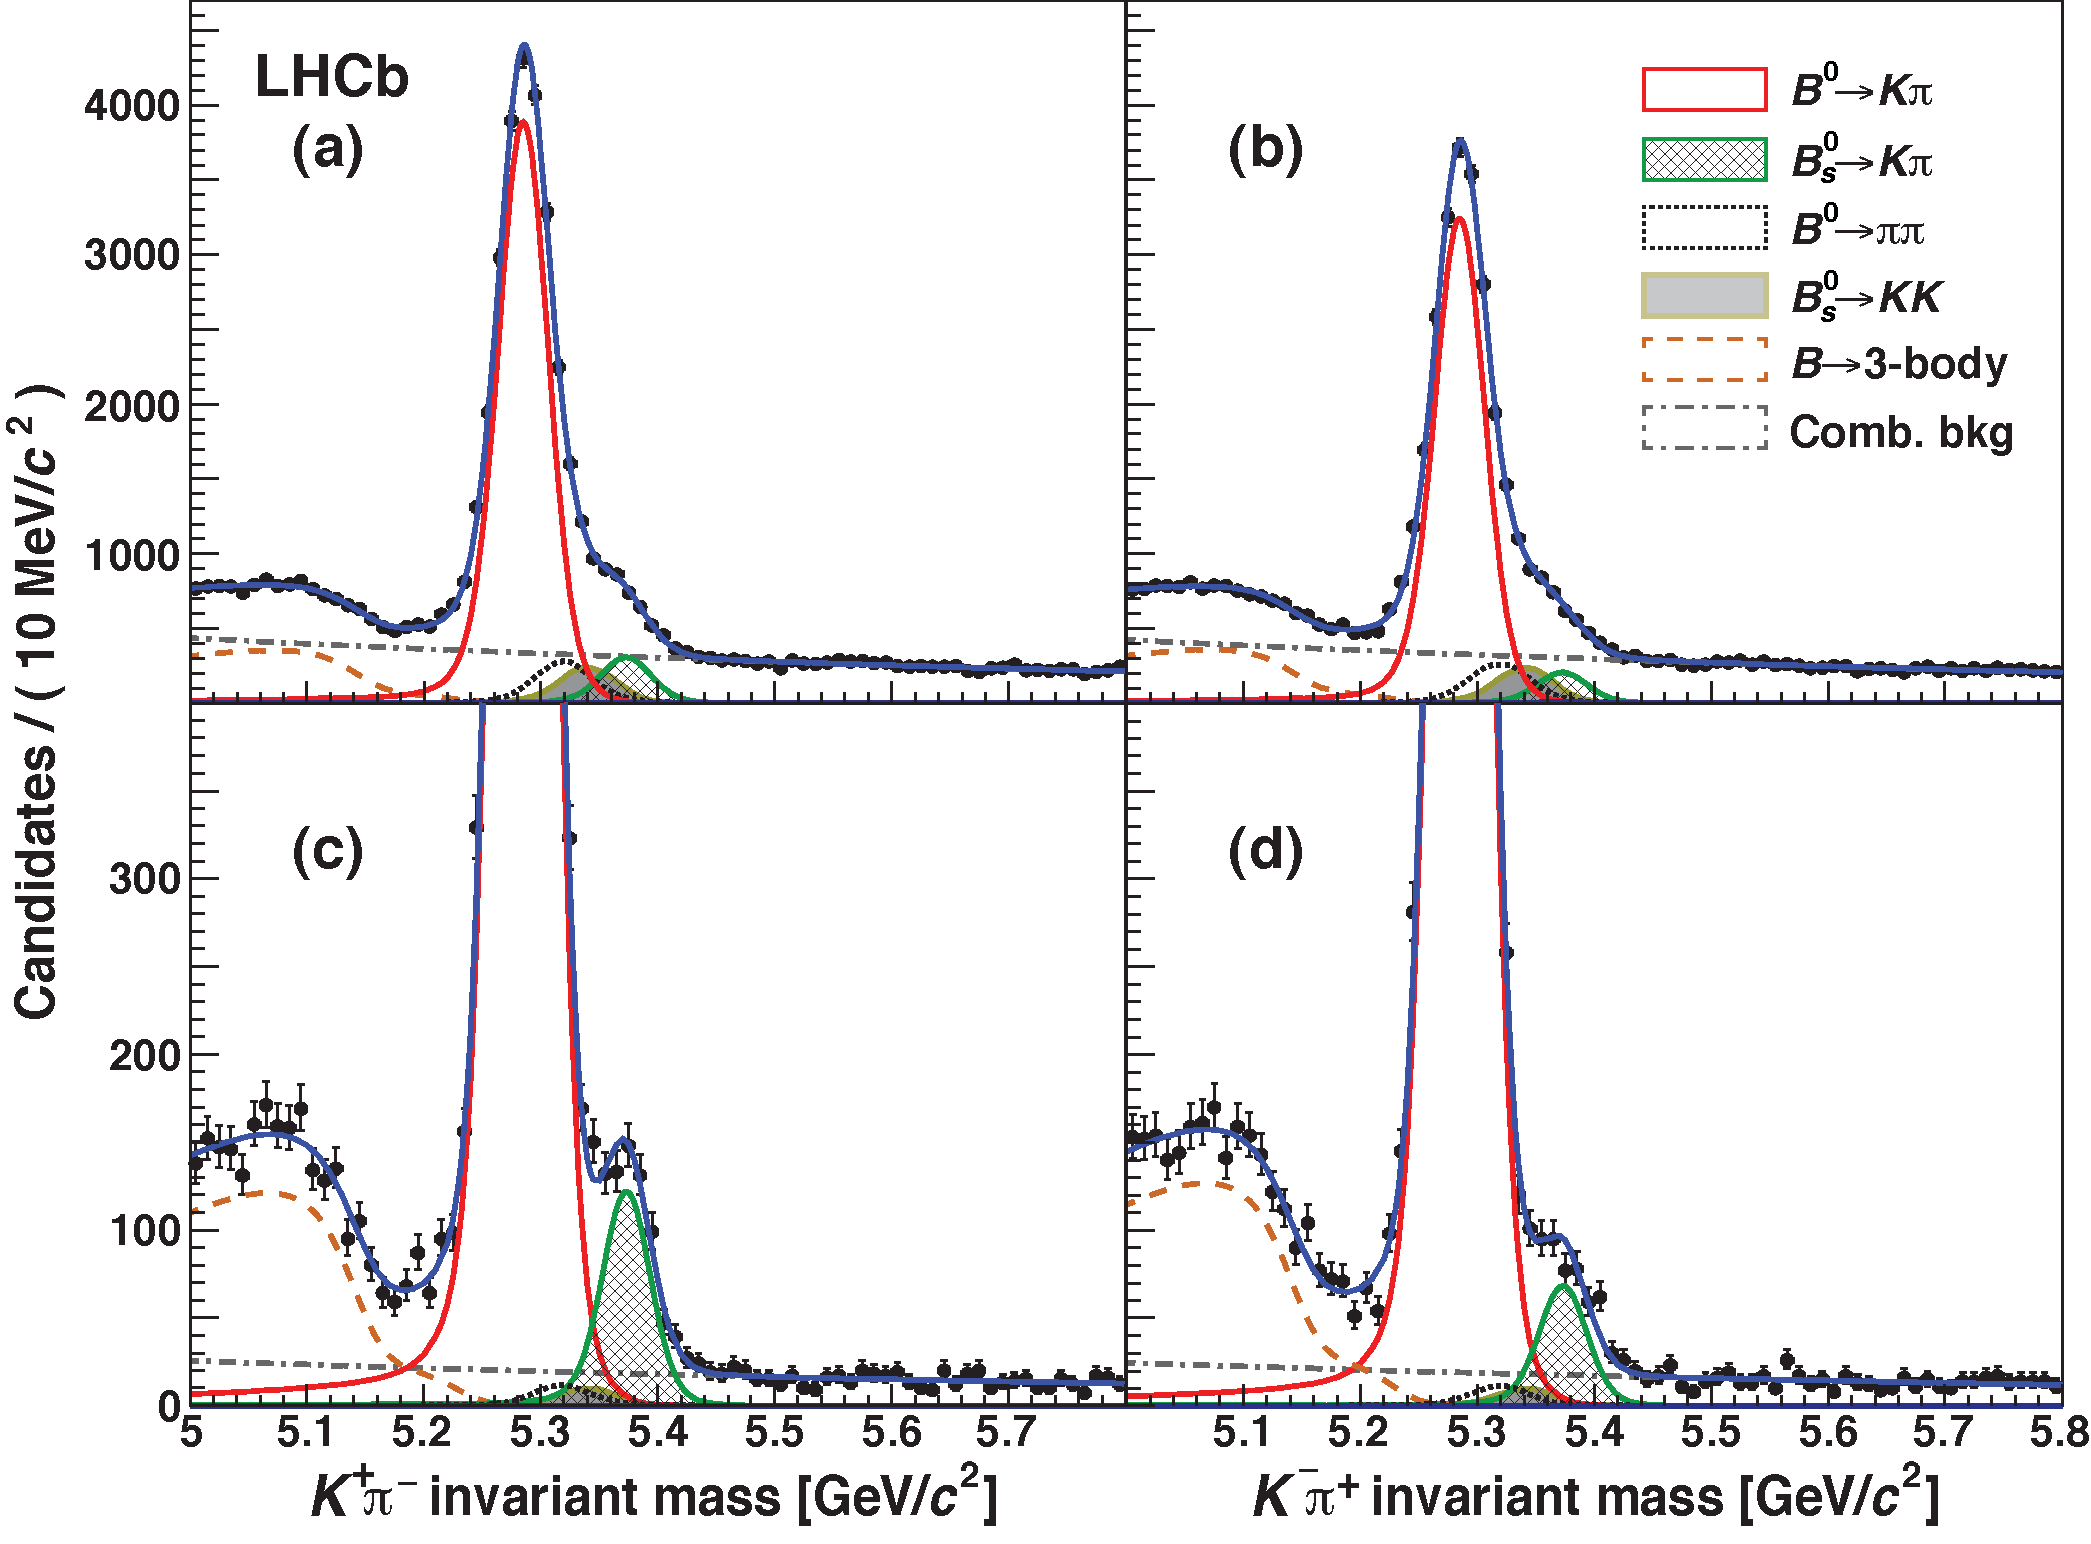
\includegraphics[width=0.8\textwidth]{03CPV/figs/DirectCPV.pdf}
	\caption{Invariant mass spectra obtained with the event selection for the best sensitivity on $A_{\CP}\left(\Bz\to\Kp\pim\right)$ (a,b) and $A_{\CP}\left(\Bs\to\Km\pip\right)$ (c,d). The figures (a) and (c) show the invariant mass distributions for \Kp\pim, figures (b) and (d) show the invariant mass distributions for \Km\pip.}
	\label{fig:DirectCPV}
\end{figure}


\subsection[head={Mixing \CP violation},tocentry={Mixing \CP violation}]{Mixing $\symbfsf{C{}P}$ violation}
\label{sec:MixingCPV}

Indirect \CP violation, also denoted as \CP violation in mixing implies that the transition probabilities for a \Bz-meson to oscilate into a \Bzb meson and vice versa are different.
As due to charge conservation mxing is only possible for uncharged mesons this type of \CP violation cannot occur for charged particles.
Using the time evolution from \cref{eq:timeEvolution} the probabilities of initially produced \Bz and \Bzb mesons to have oscillated within a proper-time $t$ are
\begin{align}
\left|\left<\Bz\Big|\Bzb\!\left(t\right)\right>\right|^2=\frac{1}{4}\left|\frac{p}{q}\right|^2
\left(e^{-\GH t}+e^{-\GL t}-2e^{\frac{1}{2}\left(\Gamma\right)t}\cos\left(\dm t\right)\right),\\
\left|\left<\Bzb\Big|\Bz\!\left(t\right)\right>\right|^2=\frac{1}{4}\left|\frac{q}{p}\right|^2
\left(e^{-\GH t}+e^{-\GL t}-2e^{\frac{1}{2}\left(\Gamma\right)t}\cos\left(\dm t\right)\right).
\end{align}
To obtain the same probabilities for both processes obviously
\begin{equation}
\left|\frac{q}{p}\right|=\left|\frac{p}{q}\right| \Rightarrow \left|\frac{q}{p}\right|=1
\end{equation}
is required.
According to \cref{eq:qoverp} this means that indirect \CP violation occurs if the matrix elements $m_{12}$ and $\Gamma_{12}$ have different complex phases.
The \CP asymmetry in case of indirect \CP violation can be defined as
\begin{equation}
A_{\CP}(t)=\frac{\Gamma\left(\Bz\to\Bzb\right) - \Gamma\left(\Bzb\to\Bz\right)}{\Gamma\left(\Bz\to\Bzb\right) + \Gamma\left(\Bzb\to\Bz\right)}
= \frac{1-\left|\nicefrac{p}{q}\right|^4}{1+\left|\nicefrac{p}{q}\right|^4}
\end{equation}
However, as neutral \B-mesons do not just oscillate but also decay this asymmetry can not be used directly to measure \CP violation in mixing.
Instead the \B-mesons need to be reconstructed in flavour specific decays, \ie only the transitions $\Bz\to\f$ and $\Bzb\to\fbar$, but not $\Bz\to\fbar$ and $\Bzb\to\f$ are allowed.
Thus the flavour of the meson at decay can be determined by final state and compared to the initial production flavour.
For the \Bz and \Bs meson system \CP violation in mixing has been measured to be negligible \cite{HFLAV2016} what is in good agreement with the \ac{SM} predictions.

\subsection[head={Interference \CP violation},tocentry={Interference \CP violation}]{Interference $\symbfsf{C{}P}$ violation}
\label{sec:InterferenceCPV}

So far \CP violation arising due to a clash between the phases of two interfering decay amplitudes or a clash between the phases of $m_{12}$ and $\Gamma_{12}$ has been discussed.
The third possibility is a clash between the phase of $\nicefrac{q}{p}$ and the phase of the decay amplitude what results in the so-called interference \CP violation.
For this class of \CP violation decays of \Bz and \Bzb mesons into both the final state \f and its \CP-conjugate \fbar need to be considered.

Inverting the requirement for \CP violation in mixing shows that \CP is conserved when there is a phase $\xi'$ such that
\begin{equation}
\begin{split}
m_{12}^\ast &= e^{2i\xi'}m_{12}\\
\Gamma_{12}^\ast &= e^{2i\xi'}\Gamma_{12}\label{eq:CPconservationMixing}
\end{split}
\end{equation}
what leads directly to $\nicefrac{q^2}{p^2} = e^{2i\xi'}$.
Using \cref{eq:CPTransInitFinal} the \CP conjugated amplitudes \Abarfbar and \Afbar can be expressed as
\begin{align}
\Abarfbar&=e^{i\left(\xi_f-\xi\right)}\Af,\label{eq:amplitudetransformation_1}\\
\Afbar&=e^{i\left(\xi_f+\xi\right)}\Abarf.\label{eq:amplitudetransformation_2}
\end{align}
what leads to $\big|\,\Af\,\big|=\big|\,\Abarfbar\,\big|$ and $\big|\,\Abarf\,\big|=\big|\,\Afbar\,\big|$ after eliminating the phases and shows that these amplitudes are \CP conserving.
Combining \cref{eq:amplitudetransformation_1} and \cref{eq:amplitudetransformation_2} then leads to
\begin{equation}
\Af\,\Afbar=e^{2i\xi}\,\Abarfbar\,\Abarf\,.
\end{equation}
Under the assumption that the phase of $\nicefrac{q}{p}$ and the phases of the decay amplitudes do not clash, \ie $\xi=\xi'$, \CP is conserved and
\begin{equation}
\arg\left(\frac{p^2}{q^2}\Af \,\overline{\kern -1.0pt A\kern -1.0pt}_{\kern 1.0pt f}^\ast\,\Afbar\overline{\kern -1.0pt \,A\kern -1.0pt}_{\kern 2.5pt\overline{\kern -1.5pt f\kern 1.5pt}}^\ast\right)=0
\end{equation}
applies.
This can be reformulated using the parameters
\begin{equation}
\Lf=\frac{q}{p}\frac{\Abarf}{\Af}\hspace{0.5cm}\text{and}
\hspace{0.5cm}\Lfbar=\frac{p}{q}\frac{\Afbar}{\Abarfbar}.
\end{equation}
Even without \CP violation in decay or mixing ($\big|\Lf\big|=\big|\Lfbar\big| = \pm1$) \CP is not conserved in case of
\begin{equation}
	\arg\left(\Lf\right)-\arg\left(\Lfbar\right)\neq0. \label{eq:conditionCPV}
\end{equation}

This type of \CP violation was first measured by the \B-factories \babar \cite{Aubert:2001nu} and \belle \cite{Abe:2001xe}.
The most prominent measurement is probably the anlysis of the so-called golden mode \BdToJPsiKS to determine $\sin{}\left(2\beta\right)$.
For this decay channel the condition in \cref{eq:conditionCPV} can be simplified to $\arg\left(\Lf\right)\neq0$ as only one common finalstate for both \Bz and \Bzb exists.
Furthermore no \CP violation in decay and mixing is expected for the decay \BdToJPsiKS and with the current experimental precision $\DG=0$ can be assumed.
Therefore the \CP asymmetry can be expressed as
\begin{equation}
A_{\CP}(t)=\frac{\Gamma\left(\BdToJPsiKS\right)-\Gamma\left(\BdToJPsiKS\right)}{\Gamma\left(\BdToJPsiKS\right)+\Gamma\left(\BdToJPsiKS\right)}=\Sf\sin\left(\dmd t\right),
\end{equation}
with the parameter $\Sf=\sin{}\left(2\beta\right)$ (a more thoroughly description of the formalism will be given in \cref{ch:CKMAngleGamma}).
The most recent measurement of \Sf was performed by \lhcb \cite{Aaij:2015vza} yielding a result of
\begin{equation}
\Sf=0.731\pm0.035\stat0.005\syst,
\end{equation}
what is consistent with the \ac{SM} expectations. The resulting \CP asymmetry is shown in \cref{fig:sin2beta}
\begin{figure}[tbp]
	\centering
	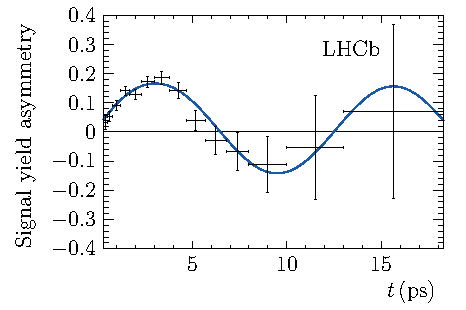
\includegraphics[width=0.6\textwidth]{03CPV/figs/InterferenceCPV.pdf}
	\caption{Time-dependent signal yield asymmetry $\left(N_{\Bzb}-N_{\Bz}\right)/\left(N_{\Bzb}-N_{\Bz}\right)$. The black points represent the used datasample, the solid curve is the projection of the signal \PDF.}
	\label{fig:sin2beta}
\end{figure}

  % !TEX root = main.tex
\chapter{The \lhcb experiment}

\blindtext

\section{The Large Hadron Collider}

\Blindtext

\section{The \lhcb detector}

\Blindtext

\subsection{The tracking system}

\subsection{The particle identification system}

\subsection{Trigger}

\subsection{The LHCb software stack}

  % !TEX root = main.tex
\chapter{Data sample and selection}

\blindtext

\section{Data sample}

\Blindtext

\section{Simulation samples}

\Blindtext

\section{Selection}

\blindtext

\subsection{Preselection and trigger requirements}

\Blindtext

\subsection{Vetoes}

\Blindtext

\subsection{Development of a MVA classifier}

\Blindtext

\subsection{BDT selection optimisation}

\Blindtext

\subsection{Multiple Candidates}

\blindtext

\subsection{Selection Performance}

\Blindtext

  % !TEX root = main.tex
\chapter{Massfit}

\blindtext

\section{Probabity densitiy functions}

\Blindtext

\section{Fit ot data}

\Blindtext

  % !TEX root = main.tex
\chapter{Flavour Tagging}

\blindtext

\section{Tagging algorithms}

\Blindtext

\section{Flavour Tagging strategy}

\Blindtext

\section{Opposite side tagging algorithms}

\Blindtext

\section{Same side tagging algorithms}

\blindtext

\subsection{Selection of Bd2JpsiKst decays}

\Blindtext

\subsection{Retraining of the SS pion tagger}

\Blindtext

\subsection{Retraining of the SS proton tagger}

\Blindtext

\subsection{Calibration portability}

  % !TEX root = main.tex
\chapter{Decay time fit}

\blindtext

\section{Fit to data}

\Blindtext

\subsection{time dependenc detector acceptance}

\Blindtext

\subsection{decay time resolution}

\Blindtext

\subsection{Extraction of CP observables}

\Blindtext

\section{Decay Time fit validation}

\Blindtext

\subsection{Fits in subsamples}

\Blindtext

\subsection{Time fits to MC Bootstrap samples}

\Blindtext

  % !TEX root = main.tex
\chapter{Systematic uncertainties}

\blindtext

\section{Systematics from Gaussian constraints}

\Blindtext

\section{Systematics from Toys}

\Blindtext

  % !TEX root = main.tex
\chapter{Results}

\Blindtext


  % !TEX root = main.tex
\chapter{Conclusion}

\Blindtext



\backmatter
  \printbibliography

\newpage
\pagestyle{empty}
% !TEX root = main.tex
\chapter{Acknowledgements}

Zuallererst möchte ich mich bei meinem Doktorvater Herrn Professor Spaan bedanken.
Nachdem er mich \num{2012} für die Bachelorarbeit am Lehrstuhl willkommen hieß, bin ich \num{2013} zur Masterarbeit zurückgekehrt und schließe nun meine Promotion \num{6} Jahre später ab.
Während dieser Zeit, haben Sie mich in allen Aufgaben unterstützt und mir einige Konferenzbesuche, sowie diverse Aufenthalte am \cern ermöglicht, die ich sicher nicht vergessen werde.

Weiterhin möchte ich Herrn Professor Kröninger danken, dass er trotz einiger anderer Dissertationen, zugestimmt hat, auch Zeit als Zweitgutachter für diese Arbeit zu finden.

A huge thank-you goes to my analysis colleagues from Dortmund and Lausanne.
Together we made this analysis possible, after some quite painful times, \eg before rushing for CKM.
A special thank goes to Julian, who supported me very strongly made it very easy for me to join the various \lhcb working group and was always there to answer questions and give advice, although I surely was not the only PhD student regularly asking him.
Also I want to say thank you to Vincenzo, who fighted with me though quite some barriers for this analysis.
Finally, not to forget Conor and Mirco: It was a pleasure to work with you, and I learned many things in fruitful discussions!

Ein Dank geht weiterhin an alle Büro- und Arbeitsgruppenkollegen, sei es aus der lokalen \enquote{\B to open charm} Arbeitsgruppe mit Frank, Philipp (vielen Dank vor allem auch an das teilweise prompte und intensive Korrekturlesen dieser Arbeit), Margarete und Ulrich (der ebenfalls mit mir am Flavour Tagging gearbeitet hat), oder aus der lokalen Flavour Tagging Arbeitsgruppe mit Kevin.
Die vielen Diskussionen haben mir immer wieder hilfreiche Anstöße gegeben.

Zur etwa gleichen Zeit haben wir zumindest die Promotion, teilweise sogar die Masterarbeit am Lehrstuhl E5 begonnen und dabei auch des öfteren mal nicht über Physik geredet und so ab und an den Kopf freibekommen: Vielen Dank an Vanessa, Timon, Moritz und Janine.

Außerdem gilt mein Dank unserer Sekretärin Frau Stickel, die mir in so manch einer bürokratischen Angelegenhet weitergeholfen hat und ohne die manch eine Abrechnung oder Dienstreise nicht so einfach abgelaufen wäre.

Schlußendlich möchte ich noch allen weiteren Lehrstuhlmitgliedern bei E5 danken für die gute, gemeinschaftliche Atmosphäre!\\
\\
Abseits der Universität möchte ich außerdem meiner Familie und dort zuallererst meinen Eltern danken, die mir das Physikstudium, und ebenfalls die anschließende Promotion durch ihre unentwegte Unterstützung ermöglicht haben.
Ebenfalls danke ich meinen beiden Brüdern, die mir immer beigestanden haben.

Zu guter Letzt geht mein Dank außerdem an Gina: Seit wir uns kennengelernt haben, hast du mich besonders immer wenn es eng und stressig wurde unterstützt, mir Aufgaben abgenommen, mich motiviert und mein Blickfeld erweitert.
Nicht zu vergessen, als erste diese Arbeit auf sprachliche Fehler zu durchsuchen, und somit allen weiteren Korrekturlesern meine gröbsten Fehltritte vorweggenommen zu haben.



\newpage
% \input{versicherung}
\end{document}

